% Options for packages loaded elsewhere
\PassOptionsToPackage{unicode}{hyperref}
\PassOptionsToPackage{hyphens}{url}
\PassOptionsToPackage{dvipsnames,svgnames,x11names}{xcolor}
%
\documentclass[
  singlecolumn]{report}

\usepackage{amsmath,amssymb}
\usepackage{iftex}
\ifPDFTeX
  \usepackage[T1]{fontenc}
  \usepackage[utf8]{inputenc}
  \usepackage{textcomp} % provide euro and other symbols
\else % if luatex or xetex
  \usepackage{unicode-math}
  \defaultfontfeatures{Scale=MatchLowercase}
  \defaultfontfeatures[\rmfamily]{Ligatures=TeX,Scale=1}
\fi
\usepackage[]{libertinus}
\ifPDFTeX\else  
    % xetex/luatex font selection
\fi
% Use upquote if available, for straight quotes in verbatim environments
\IfFileExists{upquote.sty}{\usepackage{upquote}}{}
\IfFileExists{microtype.sty}{% use microtype if available
  \usepackage[]{microtype}
  \UseMicrotypeSet[protrusion]{basicmath} % disable protrusion for tt fonts
}{}
\makeatletter
\@ifundefined{KOMAClassName}{% if non-KOMA class
  \IfFileExists{parskip.sty}{%
    \usepackage{parskip}
  }{% else
    \setlength{\parindent}{0pt}
    \setlength{\parskip}{6pt plus 2pt minus 1pt}}
}{% if KOMA class
  \KOMAoptions{parskip=half}}
\makeatother
\usepackage{xcolor}
\usepackage[top=30mm,left=20mm,heightrounded]{geometry}
\setlength{\emergencystretch}{3em} % prevent overfull lines
\setcounter{secnumdepth}{-\maxdimen} % remove section numbering
% Make \paragraph and \subparagraph free-standing
\ifx\paragraph\undefined\else
  \let\oldparagraph\paragraph
  \renewcommand{\paragraph}[1]{\oldparagraph{#1}\mbox{}}
\fi
\ifx\subparagraph\undefined\else
  \let\oldsubparagraph\subparagraph
  \renewcommand{\subparagraph}[1]{\oldsubparagraph{#1}\mbox{}}
\fi


\providecommand{\tightlist}{%
  \setlength{\itemsep}{0pt}\setlength{\parskip}{0pt}}\usepackage{longtable,booktabs,array}
\usepackage{calc} % for calculating minipage widths
% Correct order of tables after \paragraph or \subparagraph
\usepackage{etoolbox}
\makeatletter
\patchcmd\longtable{\par}{\if@noskipsec\mbox{}\fi\par}{}{}
\makeatother
% Allow footnotes in longtable head/foot
\IfFileExists{footnotehyper.sty}{\usepackage{footnotehyper}}{\usepackage{footnote}}
\makesavenoteenv{longtable}
\usepackage{graphicx}
\makeatletter
\def\maxwidth{\ifdim\Gin@nat@width>\linewidth\linewidth\else\Gin@nat@width\fi}
\def\maxheight{\ifdim\Gin@nat@height>\textheight\textheight\else\Gin@nat@height\fi}
\makeatother
% Scale images if necessary, so that they will not overflow the page
% margins by default, and it is still possible to overwrite the defaults
% using explicit options in \includegraphics[width, height, ...]{}
\setkeys{Gin}{width=\maxwidth,height=\maxheight,keepaspectratio}
% Set default figure placement to htbp
\makeatletter
\def\fps@figure{htbp}
\makeatother
\newlength{\cslhangindent}
\setlength{\cslhangindent}{1.5em}
\newlength{\csllabelwidth}
\setlength{\csllabelwidth}{3em}
\newlength{\cslentryspacingunit} % times entry-spacing
\setlength{\cslentryspacingunit}{\parskip}
\newenvironment{CSLReferences}[2] % #1 hanging-ident, #2 entry spacing
 {% don't indent paragraphs
  \setlength{\parindent}{0pt}
  % turn on hanging indent if param 1 is 1
  \ifodd #1
  \let\oldpar\par
  \def\par{\hangindent=\cslhangindent\oldpar}
  \fi
  % set entry spacing
  \setlength{\parskip}{#2\cslentryspacingunit}
 }%
 {}
\usepackage{calc}
\newcommand{\CSLBlock}[1]{#1\hfill\break}
\newcommand{\CSLLeftMargin}[1]{\parbox[t]{\csllabelwidth}{#1}}
\newcommand{\CSLRightInline}[1]{\parbox[t]{\linewidth - \csllabelwidth}{#1}\break}
\newcommand{\CSLIndent}[1]{\hspace{\cslhangindent}#1}

\usepackage{booktabs}
\usepackage{longtable}
\usepackage{array}
\usepackage{multirow}
\usepackage{wrapfig}
\usepackage{float}
\usepackage{colortbl}
\usepackage{pdflscape}
\usepackage{tabu}
\usepackage{threeparttable}
\usepackage{threeparttablex}
\usepackage[normalem]{ulem}
\usepackage{makecell}
\usepackage{xcolor}
\usepackage{cancel}
\makeatletter
\makeatother
\makeatletter
\makeatother
\makeatletter
\@ifpackageloaded{caption}{}{\usepackage{caption}}
\AtBeginDocument{%
\ifdefined\contentsname
  \renewcommand*\contentsname{Table of contents}
\else
  \newcommand\contentsname{Table of contents}
\fi
\ifdefined\listfigurename
  \renewcommand*\listfigurename{List of Figures}
\else
  \newcommand\listfigurename{List of Figures}
\fi
\ifdefined\listtablename
  \renewcommand*\listtablename{List of Tables}
\else
  \newcommand\listtablename{List of Tables}
\fi
\ifdefined\figurename
  \renewcommand*\figurename{Figure}
\else
  \newcommand\figurename{Figure}
\fi
\ifdefined\tablename
  \renewcommand*\tablename{Table}
\else
  \newcommand\tablename{Table}
\fi
}
\@ifpackageloaded{float}{}{\usepackage{float}}
\floatstyle{ruled}
\@ifundefined{c@chapter}{\newfloat{codelisting}{h}{lop}}{\newfloat{codelisting}{h}{lop}[chapter]}
\floatname{codelisting}{Listing}
\newcommand*\listoflistings{\listof{codelisting}{List of Listings}}
\makeatother
\makeatletter
\@ifpackageloaded{caption}{}{\usepackage{caption}}
\@ifpackageloaded{subcaption}{}{\usepackage{subcaption}}
\makeatother
\makeatletter
\@ifpackageloaded{tcolorbox}{}{\usepackage[skins,breakable]{tcolorbox}}
\makeatother
\makeatletter
\@ifundefined{shadecolor}{\definecolor{shadecolor}{rgb}{.97, .97, .97}}
\makeatother
\makeatletter
\makeatother
\makeatletter
\makeatother
\ifLuaTeX
  \usepackage{selnolig}  % disable illegal ligatures
\fi
\IfFileExists{bookmark.sty}{\usepackage{bookmark}}{\usepackage{hyperref}}
\IfFileExists{xurl.sty}{\usepackage{xurl}}{} % add URL line breaks if available
\urlstyle{same} % disable monospaced font for URLs
\hypersetup{
  pdftitle={Causal Effect of extraversion on multi-dimensionsal well-being},
  pdfauthor={Zoe Greer; Chris G. Sibley; Joseph A. Bulbulia},
  pdfkeywords={measurement},
  colorlinks=true,
  linkcolor={blue},
  filecolor={Maroon},
  citecolor={Blue},
  urlcolor={Blue},
  pdfcreator={LaTeX via pandoc}}

\title{Causal Effect of extraversion on multi-dimensionsal well-being}
\author{Zoe Greer \and Chris G. Sibley \and Joseph A. Bulbulia}
\date{2023-07-09}

\begin{document}
\maketitle
\begin{abstract}
We combine national panel data with a potential outcomes framework to
estimate the causal effects of extraversion on multidimensional
well-being. We find evidence for a one-year causal effect of
extraversion on many domains for psychological and especially social
well-being, although with no evidence for causal effects on health.
\end{abstract}
\ifdefined\Shaded\renewenvironment{Shaded}{\begin{tcolorbox}[borderline west={3pt}{0pt}{shadecolor}, sharp corners, boxrule=0pt, frame hidden, interior hidden, enhanced, breakable]}{\end{tcolorbox}}\fi

\listoffigures
\listoftables
\hypertarget{introduction}{%
\section{Introduction}\label{introduction}}

There is correlational research that showing that extraversion is
correlated with well-being. Evidence for causality, however, is scarce.

\hypertarget{method}{%
\section{Method}\label{method}}

\begin{itemize}
\tightlist
\item
  We apply doubly-robust estimators to longitudinal data from the the
  New Zealand Attitudes and Values Study
  (\protect\hyperlink{ref-sibley2021}{Chris G. Sibley 2021}) waves
  10-12.
\item
  We measure extraversion using the Mini-IPIP6
  (\protect\hyperlink{ref-sibley2011}{Chris G. Sibley et al. 2011})
\item
  To assess causality we require a causal estimand: ``what would happen
  if?''
\item
  We use the target-trial framework following Miguel A. Hernán et al.
  (\protect\hyperlink{ref-hernuxe1n2016}{2016}) to consider the
  hypothetical causal effect of shifting the population from the second
  quartile on extraversion to the fourth quartile
  (\protect\hyperlink{ref-hernuxe1n2022}{Miguel A. Hernán, Wang, and
  Leaf 2022}; \protect\hyperlink{ref-bulbulia2022}{J. A. Bulbulia 2022};
  \protect\hyperlink{ref-hernan2023}{Hernan and Robins 2023}). This
  estimand in interesting because it has practical implications. If we
  could intervene on people with relatively low extraversion to
  relatively high extra-version, what would be the outcome across
  multi-dimensional well-being?
\item
  We consider multi-dimensional well-being following VanderWeele,
  Mathur, and Chen (\protect\hyperlink{ref-vanderweele2020}{2020})
  outcome-wide model, to improve scientific understanding while avoiding
  selectivity in measures of well-being.
\end{itemize}

\hypertarget{selection-criteria}{%
\subsection{Selection criteria}\label{selection-criteria}}

\begin{itemize}
\tightlist
\item
  Enrolled in NZAVS in 2018 and 2019.
\item
  Responded to extraversion items in 2018 and 2019.
\item
  Could be lost to follow up in 2020 (missing data multiply imputed).
\item
  Missing data permitted in all other indicators (multiply imputed).
\item
  Sample \(N\) = 34189
\end{itemize}

Figure~\ref{fig-outcomewide-dag} presents the three-wave design for
causal inference. By including indicators of the both the exposure and
outcome at baseline, any unmeasured confounder of the exposure (+1
baseline) and outcome (+2 baseline) would need to be orthogonal to the
baseline indicators. Although our approach offers a powerful means for
controlling unmeasured confounding, because we cannot ensure balance, we
peform sensitivity analysis by evaluating E-values. E-values represent
the minimum strength of association on the Risk-Ratio scale that an
unmeasured confounder would need to have with both treatment and outcome
in order to explain the observed effect estimates conditional on
measured covariates
(\protect\hyperlink{ref-vanderweele2017}{\textbf{vanderweele2017?}}).
E-values for all outcomes are reported in the tables and graphs below.

\begin{figure}

{\centering \includegraphics[width=0.8\textwidth,height=\textheight]{extroversion_files/figure-pdf/fig-outcomewide-dag-1.pdf}

}

\caption{\label{fig-outcomewide-dag}Causal graph: three-wave panel
design with selection bias}

\end{figure}

\hypertarget{selection-bias}{%
\subsection{Selection Bias}\label{selection-bias}}

To avoid selection bias from non-response and attrition bias, we
multiply imputed missing data as presented in Figure~\ref{fig-dag}. We
perform multiple imputation \emph{separately} within each qauartile of
extraversion, and combine the imputations after modelling missingness
conditional on the observed covariates (see:
(\protect\hyperlink{ref-zhang2023}{Zhang et al. 2023};
\protect\hyperlink{ref-westreich2015}{Westreich et al. 2015})). We
implement multiple imputation using the \texttt{mice} package in R
(\protect\hyperlink{ref-vanbuuren2018}{Van Buuren 2018}). We imputed 10
x missing data sets which were passed separately to the the
\texttt{MatchThem} and \texttt{WeightIt} packages to obtain exposure
weights (akin to propensity scores).

\begin{figure}

{\centering 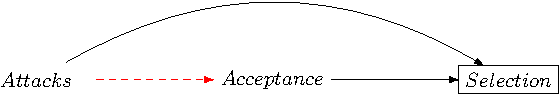
\includegraphics[width=0.8\textwidth,height=\textheight]{extroversion_files/figure-pdf/fig-dag-1.pdf}

}

\caption{\label{fig-dag}Causal graph shows potential for selection bias
from loss to follow up or non-response. To address this, we multiply
impute missing values conditional on the assumption that missing values
are random conditional on the imputation model (MAR).}

\end{figure}

\hypertarget{assssing-positivity}{%
\subsection{Assssing positivity}\label{assssing-positivity}}

To evaluation causality requires that the intervention is plausible. Can
extraversion change? To evaluate this question we assessed evidence for
movement between different levels of extraversion between NZAVS wave 10
and wave 11.

\hypertarget{tbl-transition-factor}{}
\begin{longtable}[]{@{}ccccc@{}}
\caption{\label{tbl-transition-factor}Transition matrix for change
stability and change extraversion by quartiles. Labels show range on 1-7
response scale}\tabularnewline
\toprule\noalign{}
From & 1\_3 & 3\_3.75 & 3.75\_4.75 & 4.75\_7 \\
\midrule\noalign{}
\endfirsthead
\toprule\noalign{}
From & 1\_3 & 3\_3.75 & 3.75\_4.75 & 4.75\_7 \\
\midrule\noalign{}
\endhead
\bottomrule\noalign{}
\endlastfoot
1\_3 & 4779 & 1748 & 570 & 65 \\
3\_3.75 & 1799 & 2956 & 2158 & 297 \\
3.75\_4.75 & 633 & 2316 & 5564 & 2046 \\
4.75\_7 & 71 & 351 & 2277 & 6559 \\
\end{longtable}

The transition matrix in Table~\ref{tbl-transition-factor} describes the
shifts from one state of extraversion to another between the baseline
wave (nzavs wave 10) and the following wave (nzavs wave 11). The numbers
in the cells represent the number of individuals who transitioned from
one state (rows) to another (columns). For example, the cell in the
first row and third column shows the number of individuals who
transitioned from the first state (indicated by the left-most cell in
the row) to the third state (n=570). The top left cell shows the number
of individuals who remained in the first state (n = 4779). Here we find
that n=297 individuals moved from the second quartile to the fourth
quartile.

Note that it is possible to estimate different causal effects. For
example, we might have asked: ``What would the causal effect be in the
population if everyone were to move between the lowest quartile and the
third quartile?''

\textbf{Note to co-authors: we can pick a different estimand.
Alternatively, we could use a continuous estimand, or report both.}

\hypertarget{inverse-probability-of-treatment-weighting}{%
\subsection{Inverse Probability of Treatment
Weighting}\label{inverse-probability-of-treatment-weighting}}

We first identified covariates for which balance is required, following
VanderWeeles modified disjunctive cause criterion
(\protect\hyperlink{ref-vanderweele2019}{VanderWeele 2019};
\protect\hyperlink{ref-vanderweele2020}{VanderWeele, Mathur, and Chen
2020}).

We used the \texttt{WeightIt} package in R
(\protect\hyperlink{ref-greifer2023a}{Greifer 2023b}) to obtain weights
for the exposure model, where the exposure was modelled as a function of
all baseline covariates. We used the \texttt{cobalt} pack to assess the
reliability of weights (\protect\hyperlink{ref-greifer2023b}{Greifer
2023a}). These weights were further augmented by post-stratification
weights for the NZAVS on age, gender, and European ethnicity (see:
(\protect\hyperlink{ref-sibley2021}{Chris G. Sibley 2021})).

We doubly robust estimator in which all outcomes measured at time +2
(NZAVS wave 12) were regressed against the exposure measured at time +1
(NZAVS wave 11) \(\times\) all baseline covariates measured at time 0
(NZAVS wave 10). weights for the exposure modelled were included in the
weighted regression. This approach follows {``Agnostic Notes on
Regression Adjustments to Experimental Data: Reexamining Freedman{'}s
Critique''} (\protect\hyperlink{ref-agnostic}{n.d.}) to obtain the
confounding control that is sensitive to model misspecification for the
outcome model or the exposure model.

We used the \texttt{Clarify}
(\protect\hyperlink{ref-greifer2023}{Greifer et al. 2023};
\protect\hyperlink{ref-king2000}{King, Tomz, and Wittenberg 2000}) in R
(\protect\hyperlink{ref-rainey2023}{Rainey 2023}) to estimate standard
errors and confidence intervals.

We note that the confidence intervals for doubly robust models such as
ours tend to be wider (we prefer variance over bias).

Figure~\ref{fig-propensity-score-example} shows example of baseline
imbalance (Here, the reflective domain). All domains reveal strong
imbalance in the baseline covariates that predict the exposure. Not
surprisingly, the strongest of these covariates pertain to the exposure
itself. This raises the important point that to access the incidence
effect, we must control for baseline exposure. Here we control both by
propensity score weighting (the exposure model) and regression
adjustment (the outcome model).\footnote{We compared trimmed propensity
  score weights with the untrimmed scores and found no difference to
  inference (\protect\hyperlink{ref-greifer2023}{Greifer et al. 2023}).
  We therefore report the raw (untrimmed) weights (\emph{Appendix to
  follow})}

\begin{figure}

{\centering \includegraphics{extroversion_files/figure-pdf/fig-propensity-score-example-1.pdf}

}

\caption{\label{fig-propensity-score-example}Evidence for strong
imbalance of covariates at baseline (red points). We use the entropy
balance method to ensure balance in baseline confounders (green
points).}

\end{figure}

\hypertarget{results}{%
\section{Results}\label{results}}

This set of results reports the hypothetical effect of intervening on
extraversion by setting the population to the lower quartile of
extraversion and increasinge extraversion to the third-quartile.
Outcomes are measured one-year after this hypothetical intervention.

\hypertarget{effects-on-health}{%
\subsection{Effects on health}\label{effects-on-health}}

\begin{figure}

{\centering 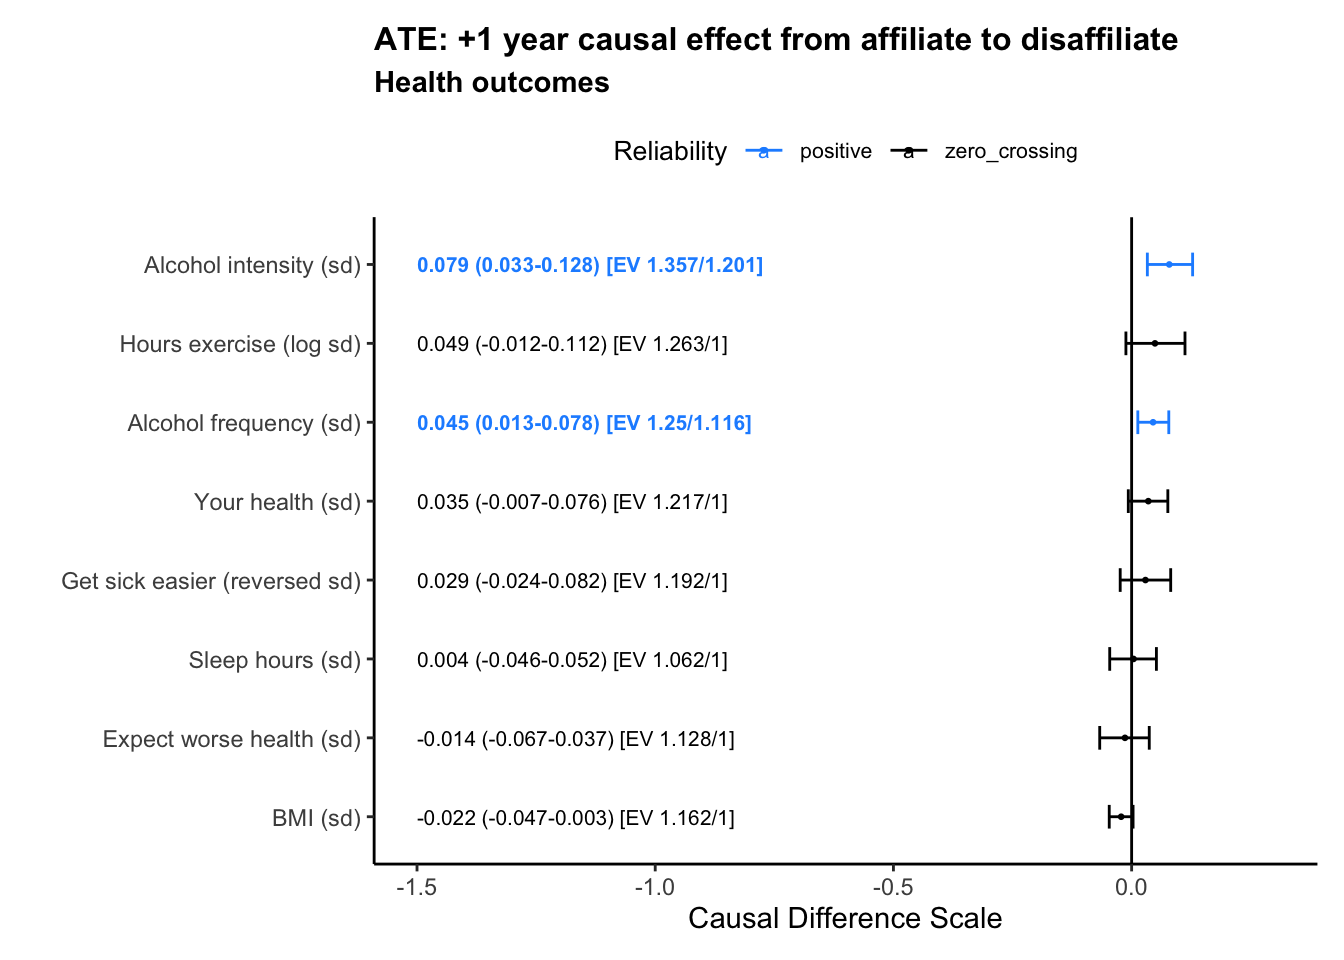
\includegraphics{extroversion_files/figure-pdf/fig-results-health-1.pdf}

}

\caption{\label{fig-results-health}Causal effects of extraversion gain
on reported physical health}

\end{figure}

Figure Figure~\ref{fig-results-health} and \textbf{?@tbl-results-health}
present the Population Average Treatment Effect (PATE). This is the
expected difference in outcomes between treatment and control groups for
the New Zealand population for the +1 year outcomes after a change in
extraversion. We do not find evidence of causal effects across the
health outcomes.Population Average Treatment Effect (PATE) represents
the expected difference in outcomes between treatment and control groups
for the New Zealand population.

For the outcome `SF Health expect worse health (sd)', the PATE causal
contrast is 0.043. The confidence interval ranges from -0.027 to 0.111.
The E-value for this outcome confirms the causal contrast is unreliable.

For the outcome `SF Health your health (sd)', the PATE causal contrast
is 0.042. The confidence interval ranges from -0.02 to 0.099. The
E-value for this outcome confirms the causal contrast is unreliable.

For the outcome `Alcohol intensity (sd)', the PATE causal contrast is
0.035. The confidence interval ranges from -0.024 to 0.093. The E-value
for this outcome confirms the causal contrast is unreliable.

For the outcome `Hlth sleep Hours (sd)', the PATE causal contrast is
-0.035. The confidence interval ranges from -0.106 to 0.029. The E-value
for this outcome confirms the causal contrast is unreliable.

For the outcome `Hlth bmi (sd)', the PATE causal contrast is -0.023. The
confidence interval ranges from -0.059 to 0.014. The E-value for this
outcome confirms the causal contrast is unreliable.

For the outcome `alcohol frequency (sd)', the PATE causal contrast is
0.023. The confidence interval ranges from -0.027 to 0.069. The E-value
for this outcome confirms the causal contrast is unreliable.

For the outcome `SF Health get sick easier (sd, reversed)', the PATE
causal contrast is 0.02. The confidence interval ranges from -0.05 to
0.095. The E-value for this outcome confirms the causal contrast is
unreliable.

For the outcome `Hours exercise (log sd)', the PATE causal contrast is
-0.005. The confidence interval ranges from -0.081 to 0.072. The E-value
for this outcome confirms the causal contrast is unreliable.

\hypertarget{effects-on-embodied-well-being}{%
\subsection{Effects on embodied
well-being}\label{effects-on-embodied-well-being}}

\begin{figure}

{\centering 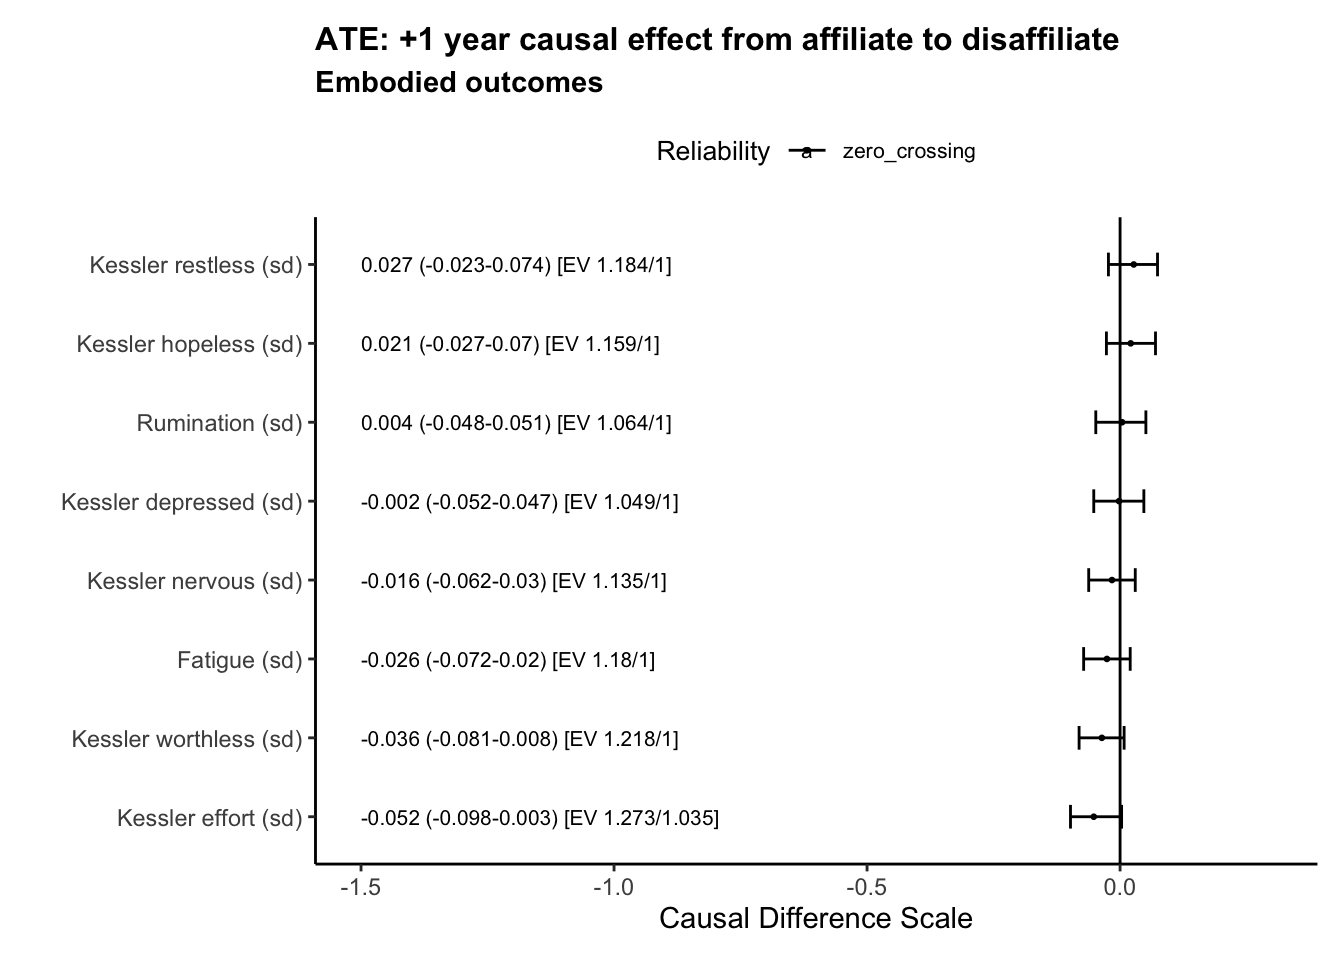
\includegraphics{extroversion_files/figure-pdf/fig-results-embodied-1.pdf}

}

\caption{\label{fig-results-embodied}Causal effects of extraversion gain
on embodied well-being}

\end{figure}

\hypertarget{tbl-results-embodied}{}
\begin{longtable}[]{@{}
  >{\raggedright\arraybackslash}p{(\columnwidth - 10\tabcolsep) * \real{0.3067}}
  >{\raggedleft\arraybackslash}p{(\columnwidth - 10\tabcolsep) * \real{0.2133}}
  >{\raggedleft\arraybackslash}p{(\columnwidth - 10\tabcolsep) * \real{0.1067}}
  >{\raggedleft\arraybackslash}p{(\columnwidth - 10\tabcolsep) * \real{0.1067}}
  >{\raggedleft\arraybackslash}p{(\columnwidth - 10\tabcolsep) * \real{0.1067}}
  >{\raggedleft\arraybackslash}p{(\columnwidth - 10\tabcolsep) * \real{0.1600}}@{}}
\caption{\label{tbl-results-embodied}Table of results for the embodied
well-being domain}\tabularnewline
\toprule\noalign{}
\begin{minipage}[b]{\linewidth}\raggedright
\end{minipage} & \begin{minipage}[b]{\linewidth}\raggedleft
E{[}Y(1){]}-E{[}Y(0){]}
\end{minipage} & \begin{minipage}[b]{\linewidth}\raggedleft
2.5 \%
\end{minipage} & \begin{minipage}[b]{\linewidth}\raggedleft
97.5 \%
\end{minipage} & \begin{minipage}[b]{\linewidth}\raggedleft
E\_Value
\end{minipage} & \begin{minipage}[b]{\linewidth}\raggedleft
E\_Val\_bound
\end{minipage} \\
\midrule\noalign{}
\endfirsthead
\toprule\noalign{}
\begin{minipage}[b]{\linewidth}\raggedright
\end{minipage} & \begin{minipage}[b]{\linewidth}\raggedleft
E{[}Y(1){]}-E{[}Y(0){]}
\end{minipage} & \begin{minipage}[b]{\linewidth}\raggedleft
2.5 \%
\end{minipage} & \begin{minipage}[b]{\linewidth}\raggedleft
97.5 \%
\end{minipage} & \begin{minipage}[b]{\linewidth}\raggedleft
E\_Value
\end{minipage} & \begin{minipage}[b]{\linewidth}\raggedleft
E\_Val\_bound
\end{minipage} \\
\midrule\noalign{}
\endhead
\bottomrule\noalign{}
\endlastfoot
Kessler worthless (sd) & -0.1529 & -0.2014 & -0.1043 & 1.563 & 1.431 \\
Kessler nervous (sd) & -0.1060 & -0.1786 & -0.0350 & 1.435 & 1.213 \\
Kessler hopeless (sd) & -0.0803 & -0.1358 & -0.0247 & 1.361 & 1.176 \\
Rumination (sd) & -0.0817 & -0.1476 & -0.0158 & 1.366 & 1.136 \\
Hlth fatigue (sd) & -0.0153 & -0.0727 & 0.0472 & 1.133 & 1.000 \\
Kessler depressed (sd) & -0.0419 & -0.1020 & 0.0194 & 1.240 & 1.000 \\
Kessler effort (sd) & -0.0439 & -0.1117 & 0.0253 & 1.247 & 1.000 \\
kessler restless (sd) & -0.0660 & -0.1339 & 0.0013 & 1.318 & 1.000 \\
\end{longtable}

Figure~\ref{fig-results-embodied} and Table~\ref{tbl-results-embodied}
presents the Population Average Treatment Effect (PATE) for the embodied
domain. We find evidence for the causal effects of change in
extraversion (from the second quartile to the fourth quartile) on five
of the six Kessler-6 dimensions, with the strong effects on feelings of
worthlessless.

For the outcome `Kessler worthless (sd)', the PATE causal contrast is
-0.153. The confidence interval ranges from -0.201 to -0.104. The
E-value for this outcome is 1.563, indicating reliable evidence for
causality.

For the outcome `Kessler nervous (sd)', the PATE causal contrast is
-0.106. The confidence interval ranges from -0.179 to -0.035. The
E-value for this outcome is 1.435, indicating reliable evidence for
causality.

For the outcome `Rumination (sd)', the PATE causal contrast is -0.082.
The confidence interval ranges from -0.148 to -0.016. The E-value for
this outcome is 1.366, indicating reliable evidence for causality.

For the outcome `Kessler hopeless (sd)', the PATE causal contrast is
-0.08. The confidence interval ranges from -0.136 to -0.025. The E-value
for this outcome is 1.361, indicating reliable evidence for causality.

For the outcome `kessler restless (sd)', the PATE causal contrast is
-0.066. The confidence interval ranges from -0.134 to 0.001. The E-value
for this outcome confirms the causal contrast is unreliable.

For the outcome `Kessler effort (sd)', the PATE causal contrast is
-0.044. The confidence interval ranges from -0.112 to 0.025. The E-value
for this outcome confirms the causal contrast is unreliable.

For the outcome `Kessler depressed (sd)', the PATE causal contrast is
-0.042. The confidence interval ranges from -0.102 to 0.019. The E-value
for this outcome confirms the causal contrast is unreliable.

For the outcome `Hlth fatigue (sd)', the PATE causal contrast is -0.015.
The confidence interval ranges from -0.073 to 0.047. The E-value for
this outcome confirms the causal contrast is unreliable.

\hypertarget{effects-on-practical-well-being}{%
\subsection{Effects on practical
well-being}\label{effects-on-practical-well-being}}

\begin{figure}

{\centering \includegraphics{extroversion_files/figure-pdf/fig-results-practical-1.pdf}

}

\caption{\label{fig-results-practical}Causal effects of extraversion
gain on practical well-being}

\end{figure}

\hypertarget{tbl-results-practical}{}
\begin{longtable}[]{@{}
  >{\raggedright\arraybackslash}p{(\columnwidth - 10\tabcolsep) * \real{0.4348}}
  >{\raggedleft\arraybackslash}p{(\columnwidth - 10\tabcolsep) * \real{0.1739}}
  >{\raggedleft\arraybackslash}p{(\columnwidth - 10\tabcolsep) * \real{0.0870}}
  >{\raggedleft\arraybackslash}p{(\columnwidth - 10\tabcolsep) * \real{0.0870}}
  >{\raggedleft\arraybackslash}p{(\columnwidth - 10\tabcolsep) * \real{0.0870}}
  >{\raggedleft\arraybackslash}p{(\columnwidth - 10\tabcolsep) * \real{0.1304}}@{}}
\caption{\label{tbl-results-practical}Table of results for the practical
well-being domain}\tabularnewline
\toprule\noalign{}
\begin{minipage}[b]{\linewidth}\raggedright
\end{minipage} & \begin{minipage}[b]{\linewidth}\raggedleft
E{[}Y(1){]}-E{[}Y(0){]}
\end{minipage} & \begin{minipage}[b]{\linewidth}\raggedleft
2.5 \%
\end{minipage} & \begin{minipage}[b]{\linewidth}\raggedleft
97.5 \%
\end{minipage} & \begin{minipage}[b]{\linewidth}\raggedleft
E\_Value
\end{minipage} & \begin{minipage}[b]{\linewidth}\raggedleft
E\_Val\_bound
\end{minipage} \\
\midrule\noalign{}
\endfirsthead
\toprule\noalign{}
\begin{minipage}[b]{\linewidth}\raggedright
\end{minipage} & \begin{minipage}[b]{\linewidth}\raggedleft
E{[}Y(1){]}-E{[}Y(0){]}
\end{minipage} & \begin{minipage}[b]{\linewidth}\raggedleft
2.5 \%
\end{minipage} & \begin{minipage}[b]{\linewidth}\raggedleft
97.5 \%
\end{minipage} & \begin{minipage}[b]{\linewidth}\raggedleft
E\_Value
\end{minipage} & \begin{minipage}[b]{\linewidth}\raggedleft
E\_Val\_bound
\end{minipage} \\
\midrule\noalign{}
\endhead
\bottomrule\noalign{}
\endlastfoot
Perfectionism (sd) & -0.1652 & -0.2189 & -0.1086 & 1.596 & 1.447 \\
Emotion reg out control (sd) & -0.1494 & -0.2139 & -0.0882 & 1.554 &
1.380 \\
Power self nocontrol (sd) & -0.1487 & -0.2178 & -0.0752 & 1.552 &
1.353 \\
Selfesteem postive self (sd) & 0.1365 & 0.0714 & 0.2036 & 1.519 &
1.332 \\
Selfesteem failure (sd, reversed) & 0.1209 & 0.0681 & 0.1757 & 1.477 &
1.322 \\
Power other control (sd) & -0.1126 & -0.1739 & -0.0511 & 1.454 &
1.272 \\
Selfesteem satself (sd) & 0.1108 & 0.0471 & 0.1742 & 1.449 & 1.259 \\
Emotion reg hide neg emotions (sd) & -0.1106 & -0.1779 & -0.0380 & 1.448
& 1.236 \\
Bodysat (sd) & 0.0898 & 0.0311 & 0.1482 & 1.389 & 1.202 \\
Vengeful rumin (sd) & -0.0754 & -0.1339 & -0.0193 & 1.347 & 1.147 \\
Sexual satisfaction (sd) & 0.0123 & -0.0474 & 0.0687 & 1.118 & 1.000 \\
Self control have lots (sd) & -0.0270 & -0.0916 & 0.0332 & 1.185 &
1.000 \\
Self control wish more (sd, reversed) & 0.0210 & -0.0367 & 0.0830 &
1.160 & 1.000 \\
Emotion reg chang thinking to calm (sd) & 0.0039 & -0.0648 & 0.0791 &
1.063 & 1.000 \\
\end{longtable}

Figure~\ref{fig-results-practical} and Table~\ref{tbl-results-practical}
present the results for practical well-being.

Population Average Treatment Effect (PATE) represents the expected
difference in outcomes between treatment and control groups for the New
Zealand population.

For the outcome `Kessler worthless (sd)', the PATE causal contrast is
-0.153. The confidence interval ranges from -0.201 to -0.104. The
E-value for this outcome is 1.563, indicating reliable evidence for
causality.

For the outcome `Kessler nervous (sd)', the PATE causal contrast is
-0.106. The confidence interval ranges from -0.179 to -0.035. The
E-value for this outcome is 1.435, indicating reliable evidence for
causality.

For the outcome `Rumination (sd)', the PATE causal contrast is -0.082.
The confidence interval ranges from -0.148 to -0.016. The E-value for
this outcome is 1.366, indicating reliable evidence for causality.

For the outcome `Kessler hopeless (sd)', the PATE causal contrast is
-0.08. The confidence interval ranges from -0.136 to -0.025. The E-value
for this outcome is 1.361, indicating reliable evidence for causality.

For the outcome `kessler restless (sd)', the PATE causal contrast is
-0.066. The confidence interval ranges from -0.134 to 0.001. The E-value
for this outcome confirms the causal contrast is unreliable.

For the outcome `Kessler effort (sd)', the PATE causal contrast is
-0.044. The confidence interval ranges from -0.112 to 0.025. The E-value
for this outcome confirms the causal contrast is unreliable.

For the outcome `Kessler depressed (sd)', the PATE causal contrast is
-0.042. The confidence interval ranges from -0.102 to 0.019. The E-value
for this outcome confirms the causal contrast is unreliable.

For the outcome `Hlth fatigue (sd)', the PATE causal contrast is -0.015.
The confidence interval ranges from -0.073 to 0.047. The E-value for
this outcome confirms the causal contrast is unreliable.

\hypertarget{effects-on-reflective-well-being}{%
\subsection{Effects on reflective
well-being}\label{effects-on-reflective-well-being}}

\begin{figure}

{\centering \includegraphics{extroversion_files/figure-pdf/fig-results-reflective-well-being-1.pdf}

}

\caption{\label{fig-results-reflective-well-being}Causal effects of
extraversion gain on reflective well-being}

\end{figure}

\hypertarget{tbl-results-reflective}{}
\begin{longtable}[]{@{}
  >{\raggedright\arraybackslash}p{(\columnwidth - 10\tabcolsep) * \real{0.3200}}
  >{\raggedleft\arraybackslash}p{(\columnwidth - 10\tabcolsep) * \real{0.2133}}
  >{\raggedleft\arraybackslash}p{(\columnwidth - 10\tabcolsep) * \real{0.1067}}
  >{\raggedleft\arraybackslash}p{(\columnwidth - 10\tabcolsep) * \real{0.0933}}
  >{\raggedleft\arraybackslash}p{(\columnwidth - 10\tabcolsep) * \real{0.1067}}
  >{\raggedleft\arraybackslash}p{(\columnwidth - 10\tabcolsep) * \real{0.1600}}@{}}
\caption{\label{tbl-results-reflective}Table of results for the
reflective well-being domain}\tabularnewline
\toprule\noalign{}
\begin{minipage}[b]{\linewidth}\raggedright
\end{minipage} & \begin{minipage}[b]{\linewidth}\raggedleft
E{[}Y(1){]}-E{[}Y(0){]}
\end{minipage} & \begin{minipage}[b]{\linewidth}\raggedleft
2.5 \%
\end{minipage} & \begin{minipage}[b]{\linewidth}\raggedleft
97.5 \%
\end{minipage} & \begin{minipage}[b]{\linewidth}\raggedleft
E\_Value
\end{minipage} & \begin{minipage}[b]{\linewidth}\raggedleft
E\_Val\_bound
\end{minipage} \\
\midrule\noalign{}
\endfirsthead
\toprule\noalign{}
\begin{minipage}[b]{\linewidth}\raggedright
\end{minipage} & \begin{minipage}[b]{\linewidth}\raggedleft
E{[}Y(1){]}-E{[}Y(0){]}
\end{minipage} & \begin{minipage}[b]{\linewidth}\raggedleft
2.5 \%
\end{minipage} & \begin{minipage}[b]{\linewidth}\raggedleft
97.5 \%
\end{minipage} & \begin{minipage}[b]{\linewidth}\raggedleft
E\_Value
\end{minipage} & \begin{minipage}[b]{\linewidth}\raggedleft
E\_Val\_bound
\end{minipage} \\
\midrule\noalign{}
\endhead
\bottomrule\noalign{}
\endlastfoot
Gratitude (sd) & 0.1869 & 0.1353 & 0.2389 & 1.654 & 1.516 \\
PWI health (sd) & -0.0081 & -0.0652 & 0.0500 & 1.094 & 1.000 \\
PWI Relationships (sd) & 0.1104 & 0.0486 & 0.1735 & 1.448 & 1.261 \\
PWI security (sd) & 0.0292 & -0.0409 & 0.0935 & 1.193 & 1.000 \\
PWI standardliving (sd) & 0.1080 & 0.0457 & 0.1696 & 1.441 & 1.254 \\
Lifesat satlife (sd) & 0.0932 & 0.0384 & 0.1477 & 1.399 & 1.228 \\
Lifesat ideal (sd) & 0.0497 & -0.0114 & 0.1096 & 1.266 & 1.000 \\
Meaning purpose (sd) & 0.1313 & 0.0715 & 0.1869 & 1.505 & 1.342 \\
Meaning sense (sd) & 0.1251 & 0.0585 & 0.1925 & 1.488 & 1.294 \\
\end{longtable}

As indicated in Figure~\ref{fig-results-reflective-well-being} and
Table~\ref{tbl-results-reflective} we do not find evidence for reliable
effects of extraversion on personal security r personal health. However,
we find evidence for effects across all other dimensions of reflective
well-being.

For the outcome `Gratitude (sd)', the PATE causal contrast is 0.187. The
confidence interval ranges from 0.138 to 0.238. The E-value for this
outcome is 1.654, indicating reliable evidence for causality.

For the outcome `Meaning sense (sd)', the PATE causal contrast is 0.128.
The confidence interval ranges from 0.054 to 0.193. The E-value for this
outcome is 1.497, indicating reliable evidence for causality.

For the outcome `Meaning purpose (sd)', the PATE causal contrast is
0.126. The confidence interval ranges from 0.066 to 0.185. The E-value
for this outcome is 1.492, indicating reliable evidence for causality.

For the outcome `PWI Relationships (sd)', the PATE causal contrast is
0.113. The confidence interval ranges from 0.064 to 0.164. The E-value
for this outcome is 1.454, indicating reliable evidence for causality.

For the outcome `PWI standard living (sd)', the PATE causal contrast is
0.099. The confidence interval ranges from 0.036 to 0.161. The E-value
for this outcome is 1.416, indicating reliable evidence for causality.

For the outcome `Lifesat satlife (sd)', the PATE causal contrast is
0.091. The confidence interval ranges from 0.037 to 0.145. The E-value
for this outcome is 1.393, indicating reliable evidence for causality.

For the outcome `Lifesat ideal (sd)', the PATE causal contrast is 0.059.
The confidence interval ranges from 0 to 0.116. The E-value for this
outcome is 1.298, indicating reliable evidence for causality.

For the outcome `PWI security (sd)', the PATE causal contrast is 0.039.
The confidence interval ranges from -0.029 to 0.104. The E-value for
this outcome confirms the causal contrast is unreliable.

For the outcome `PWI health (sd)', the PATE causal contrast is -0.001.
The confidence interval ranges from -0.057 to 0.053. The E-value for
this outcome confirms the causal contrast is unreliable.

\hypertarget{effects-social-well-being}{%
\subsection{Effects social well-being}\label{effects-social-well-being}}

\begin{figure}

{\centering \includegraphics{extroversion_files/figure-pdf/fig-results-social-wellbeing-1.pdf}

}

\caption{\label{fig-results-social-wellbeing}Causal effects of
extraversion gain on social well-being}

\end{figure}

\hypertarget{tbl-results-social}{}
\begin{longtable}[]{@{}
  >{\raggedright\arraybackslash}p{(\columnwidth - 10\tabcolsep) * \real{0.4000}}
  >{\raggedleft\arraybackslash}p{(\columnwidth - 10\tabcolsep) * \real{0.1882}}
  >{\raggedleft\arraybackslash}p{(\columnwidth - 10\tabcolsep) * \real{0.0941}}
  >{\raggedleft\arraybackslash}p{(\columnwidth - 10\tabcolsep) * \real{0.0824}}
  >{\raggedleft\arraybackslash}p{(\columnwidth - 10\tabcolsep) * \real{0.0941}}
  >{\raggedleft\arraybackslash}p{(\columnwidth - 10\tabcolsep) * \real{0.1412}}@{}}
\caption{\label{tbl-results-social}Table of results for the social
well-being domain}\tabularnewline
\toprule\noalign{}
\begin{minipage}[b]{\linewidth}\raggedright
\end{minipage} & \begin{minipage}[b]{\linewidth}\raggedleft
E{[}Y(1){]}-E{[}Y(0){]}
\end{minipage} & \begin{minipage}[b]{\linewidth}\raggedleft
2.5 \%
\end{minipage} & \begin{minipage}[b]{\linewidth}\raggedleft
97.5 \%
\end{minipage} & \begin{minipage}[b]{\linewidth}\raggedleft
E\_Value
\end{minipage} & \begin{minipage}[b]{\linewidth}\raggedleft
E\_Val\_bound
\end{minipage} \\
\midrule\noalign{}
\endfirsthead
\toprule\noalign{}
\begin{minipage}[b]{\linewidth}\raggedright
\end{minipage} & \begin{minipage}[b]{\linewidth}\raggedleft
E{[}Y(1){]}-E{[}Y(0){]}
\end{minipage} & \begin{minipage}[b]{\linewidth}\raggedleft
2.5 \%
\end{minipage} & \begin{minipage}[b]{\linewidth}\raggedleft
97.5 \%
\end{minipage} & \begin{minipage}[b]{\linewidth}\raggedleft
E\_Value
\end{minipage} & \begin{minipage}[b]{\linewidth}\raggedleft
E\_Val\_bound
\end{minipage} \\
\midrule\noalign{}
\endhead
\bottomrule\noalign{}
\endlastfoot
Belong\_outsider (sd, reversed) & 0.2794 & 0.2130 & 0.3441 & 1.900 &
1.726 \\
Belong accept (sd) & 0.1629 & 0.1017 & 0.2218 & 1.590 & 1.427 \\
Support noguidance (sd, reversed) & 0.1493 & 0.0874 & 0.2119 & 1.554 &
1.382 \\
Neighbourhood community (sd) & 0.1440 & 0.0811 & 0.2048 & 1.540 &
1.367 \\
Belong beliefs (sd) & 0.1179 & 0.0540 & 0.1875 & 1.468 & 1.272 \\
Permeability individual (sd) & 0.1041 & 0.0338 & 0.1715 & 1.430 &
1.217 \\
Support help (sd) & 0.0905 & 0.0238 & 0.1542 & 1.391 & 1.178 \\
Support turnto (sd) & 0.0829 & 0.0145 & 0.1495 & 1.369 & 1.134 \\
Impermeability group (sd) & -0.0258 & -0.0958 & 0.0472 & 1.180 &
1.000 \\
\end{longtable}

As indicated in Figure~\ref{fig-results-social-wellbeing} and
Table~\ref{tbl-results-social}, we find evidence for a causal effect of
change in extraversion across all social outcomes, with the strongest
evidence for buffering against feelings of being an outsider.

For the outcome `Belong\_outsider (sd, reversed)', the PATE causal
contrast is 0.279. The confidence interval ranges from 0.213 to 0.344.
The E-value for this outcome is 1.9, indicating reliable evidence for
causality.

For the outcome `Belong accept (sd)', the PATE causal contrast is 0.163.
The confidence interval ranges from 0.102 to 0.222. The E-value for this
outcome is 1.59, indicating reliable evidence for causality.

For the outcome `Support noguidance (sd, reversed)', the PATE causal
contrast is 0.149. The confidence interval ranges from 0.087 to 0.212.
The E-value for this outcome is 1.554, indicating reliable evidence for
causality.

For the outcome `Neighbourhood community (sd)', the PATE causal contrast
is 0.144. The confidence interval ranges from 0.081 to 0.205. The
E-value for this outcome is 1.54, indicating reliable evidence for
causality.

For the outcome `Belong beliefs (sd)', the PATE causal contrast is
0.118. The confidence interval ranges from 0.054 to 0.188. The E-value
for this outcome is 1.468, indicating reliable evidence for causality.

For the outcome `Permeability individual (sd)', the PATE causal contrast
is 0.104. The confidence interval ranges from 0.034 to 0.172. The
E-value for this outcome is 1.43, indicating reliable evidence for
causality.

For the outcome `Support help (sd)', the PATE causal contrast is 0.09.
The confidence interval ranges from 0.024 to 0.154. The E-value for this
outcome is 1.391, indicating reliable evidence for causality.

For the outcome `Support turnto (sd)', the PATE causal contrast is
0.083. The confidence interval ranges from 0.015 to 0.15. The E-value
for this outcome is 1.369, indicating reliable evidence for causality.

For the outcome `Impermeability group (sd)' -- our negative control --
the PATE causal contrast is -0.026. The confidence interval ranges from
-0.096 to 0.047. The E-value for this outcome confirms the causal
contrast is unreliable.

\hypertarget{discussion}{%
\section{Discussion}\label{discussion}}

\hypertarget{importance}{%
\subsection{Importance}\label{importance}}

\begin{itemize}
\tightlist
\item
  By emulating an experiment, we may use panel data to infer causal
  effects.
\item
  We find evidence for a causal effect of extraversion on psychological
  well-being, but not health.
\item
  This suggests that extraversion may be benefitting to psychological
  well-being.
\end{itemize}

\hypertarget{limitations}{%
\subsection{Limitations}\label{limitations}}

\begin{itemize}
\tightlist
\item
  Measurement is a limitation. Perhaps there are different types of
  extraversion.
\end{itemize}

\hypertarget{future-work}{%
\section{Future work}\label{future-work}}

\begin{itemize}
\tightlist
\item
  Pathways by which extraversion affects people remain unclear. The fact
  that people are more satisified with their personal incomes suggests
  possible pathways through employment.
\item
  Measurement of social and behavioural pathways important.
\end{itemize}

\newpage{}

\newpage{}

\hypertarget{appendix-a.-measures}{%
\section{Appendix A. Measures}\label{appendix-a.-measures}}

\hypertarget{baseline-confounding-control}{%
\subsection{Baseline confounding
control}\label{baseline-confounding-control}}

\hypertarget{age-waves-1-15}{%
\subsubsection{Age (waves: 1-15)}\label{age-waves-1-15}}

We asked participants' age in an open-ended question (``What is your
age?'' or ``What is your date of birth'').

\hypertarget{disability-waves-5-15}{%
\subsubsection{Disability (waves: 5-15)}\label{disability-waves-5-15}}

We assessed disability with a one item indicator adapted from Verbrugge
(\protect\hyperlink{ref-verbrugge1997}{1997}), that asks ``Do you have a
health condition or disability that limits you, and that has lasted for
6+ months?'' (1 = Yes, 0 = No).

\hypertarget{education-attainment-waves-1-4-15}{%
\subsubsection{Education Attainment (waves: 1,
4-15)}\label{education-attainment-waves-1-4-15}}

Participants were asked ``What is your highest level of
qualification?''. We coded participans highest finished degree according
to the New Zealand Qualifications Authority. Ordinal-Rank 0-10 NZREG
codes (with overseas school quals coded as Level 3, and all other
ancillary categories coded as missing)
See:https://www.nzqa.govt.nz/assets/Studying-in-NZ/New-Zealand-Qualification-Framework/requirements-nzqf.pdf

\hypertarget{employment-waves-1-3-4-11}{%
\subsubsection{Employment (waves: 1-3,
4-11)}\label{employment-waves-1-3-4-11}}

We asked participants ``Are you currently employed? (This includes
self-employed or casual work)''. * note: This question disappeared in
the updated NZAVS Technical documents (Data Dictionary).

\hypertarget{european-waves-1-15}{%
\subsubsection{European (waves: 1-15)}\label{european-waves-1-15}}

Participants were asked ``Which ethnic group do you belong to (NZ census
question)?'' or ``Which ethnic group(s) do you belong to? (Open-ended)''
(wave: 3). Europeans were coded as 1, whereas other ethnicities were
coded as 0.

\hypertarget{ethnicity-waves-3}{%
\subsubsection{Ethnicity (waves: 3)}\label{ethnicity-waves-3}}

Based on the New Zealand Cencus, we asked participants ``Which ethnic
group(s) do you belong to?''. The responses were: (1) New Zealand
European; (2) Māori; (3) Samoan; (4) Cook Island Māori; (5) Tongan; (6)
Niuean; (7) Chinese; (8) Indian; (9) Other such as DUTCH, JAPANESE,
TOKELAUAN. Please state:. We coded their answers into four groups:
Maori, Pacific, Asian, and Euro (except for Time 3, which used an
open-ended measure).

\hypertarget{gender-waves-1-15}{%
\subsubsection{Gender (waves: 1-15)}\label{gender-waves-1-15}}

We asked participants' gender in an open-ended question: ``what is your
gender?'' or ``Are you male or female?'' (waves: 1-5). Female was coded
as 0, Male was coded as 1, and gender diverse coded as 3
(\protect\hyperlink{ref-fraser_coding_2020}{Fraser et al. 2020}). (or
0.5 = neither female nor male)

\hypertarget{income-waves-1-3-4-15}{%
\subsubsection{Income (waves: 1-3, 4-15)}\label{income-waves-1-3-4-15}}

Participants were asked ``Please estimate your total household income
(before tax) for the year XXXX''. To stablise this indicator, we first
took the natural log of the response + 1, and then centred and
standardised the log-transformed indicator.

\hypertarget{job-security-waves-1-34-79-15}{%
\subsubsection{Job Security (waves:
1-3,4-7,9-15)}\label{job-security-waves-1-34-79-15}}

Participants indicated their feeling of job security by answering ``How
secure do you feel in your current job?'' on a scale from 1 (not secure)
to 7 (very secure).

\hypertarget{parent-waves-5-15}{%
\subsubsection{Parent (waves: 5-15)}\label{parent-waves-5-15}}

Participants were asked ``If you are a parent, what is the birth date of
your eldest child?'' or ``If you are a parent, in which year was your
eldest child born?'' (waves: 10-15). Parents were coded as 1, while the
others were coded as 0.

\hypertarget{number-of-children-waves-1-3-4-15}{%
\subsubsection{Number of Children (waves: 1-3,
4-15)}\label{number-of-children-waves-1-3-4-15}}

We measured number of children using one item from S. Bulbulia J. A.
(\protect\hyperlink{ref-Bulbulia_2015}{2015}). We asked participants
``How many children have you given birth to, fathered, or adopted. How
many children have you given birth to, fathered, or adopted?'' or
````How many children have you given birth to, fathered, or adopted. How
many children have you given birth to, fathered, and/or parented?''
(waves: 12-15).

\hypertarget{political-orientation}{%
\subsubsection{Political Orientation}\label{political-orientation}}

We measured participants' political orientation using a single item
adapted from Jost (\protect\hyperlink{ref-jost_end_2006-1}{2006}).

``Please rate how politically liberal versus conservative you see
yourself as being.''

(1 = Extremely Liberal to 7 = Extremely Conservative)

\hypertarget{nzsei-13-waves-8-15}{%
\subsubsection{NZSEI-13 (waves: 8-15)}\label{nzsei-13-waves-8-15}}

We assessed occupational prestige and status using the New Zealand
Socio-economic Index 13 (NZSEI-13)
(\protect\hyperlink{ref-fahy2017}{Fahy, Lee, and Milne 2017}). This
index uses the income, age, and education of a reference group, in this
case the 2013 New Zealand census, to calculate an score for each
occupational group. Scores range from 10 (Lowest) to 90 (Highest). This
list of index scores for occupational groups was used to assign each
participant a NZSEI-13 score based on their occupation.

Participants were asked ``If you are a parent, what is the birth date of
your eldest child?''.

\hypertarget{living-with-partner}{%
\subsubsection{Living with Partner}\label{living-with-partner}}

Participants were asekd ``Do you live with your partner?'' (1 = Yes, 0 =
No).

\hypertarget{living-in-an-urban-area-waves-1-15}{%
\subsubsection{Living in an Urban Area (waves:
1-15)}\label{living-in-an-urban-area-waves-1-15}}

We coded whether they are living in an urban or rural area (1 = Urban, 0
= Rural) based on the addresses provided.

We coded whether they are living in an urban or rural area (1 = Urban, 0
= Rural) based on the addresses provided.

\hypertarget{nz-deprivation-index-waves-1-15}{%
\subsubsection{NZ Deprivation Index (waves:
1-15)}\label{nz-deprivation-index-waves-1-15}}

We used the NZ Deprivation Index to assign each participant a score
based on where they live (\protect\hyperlink{ref-atkinson2019}{Atkinson,
Salmond, and Crampton 2019}). This score combines data such as income,
home ownership, employment, qualifications, family structure, housing,
and access to transport and communication for an area into one
deprivation score.

\hypertarget{nz-born-waves-1-24-15}{%
\subsubsection{NZ-Born (waves: 1-2,4-15)}\label{nz-born-waves-1-24-15}}

We asked participants ``Which country were you born in?'' or ``Where
were you born? (please be specific, e.g., which town/city?)'' (waves:
6-15).

\hypertarget{mini-ipip-6-waves-1-34-15}{%
\subsubsection{Mini-IPIP 6 (waves:
1-3,4-15)}\label{mini-ipip-6-waves-1-34-15}}

We measured participants personality with the Mini International
Personality Item Pool 6 (Mini-IPIP6)
(\protect\hyperlink{ref-sibley2011}{Chris G. Sibley et al. 2011}) which
consists of six dimensions and each dimensions is measured with four
items:

\begin{enumerate}
\def\labelenumi{\arabic{enumi}.}
\item
  agreeableness,

  \begin{enumerate}
  \def\labelenumii{\roman{enumii}.}
  \tightlist
  \item
    I sympathize with others' feelings.
  \item
    I am not interested in other people's problems. (r)
  \item
    I feel others' emotions.
  \item
    I am not really interested in others. (r)
  \end{enumerate}
\item
  conscientiousness,

  \begin{enumerate}
  \def\labelenumii{\roman{enumii}.}
  \tightlist
  \item
    I get chores done right away.
  \item
    I like order.
  \item
    I make a mess of things. (r)
  \item
    I ften forget to put things back in their proper place. (r)
  \end{enumerate}
\item
  extraversion,

  \begin{enumerate}
  \def\labelenumii{\roman{enumii}.}
  \tightlist
  \item
    I am the life of the party.
  \item
    I don't talk a lot. (r)
  \item
    I keep in the background. (r)
  \item
    I talk to a lot of different people at parties.
  \end{enumerate}
\item
  honesty-humility,

  \begin{enumerate}
  \def\labelenumii{\roman{enumii}.}
  \tightlist
  \item
    I feel entitled to more of everything. (r)
  \item
    I deserve more things in life. (r)
  \item
    I would like to be seen driving around in a very expensive car. (r)
  \item
    I would get a lot of pleasure from owning expensive luxury goods.
    (r)
  \end{enumerate}
\item
  neuroticism, and

  \begin{enumerate}
  \def\labelenumii{\roman{enumii}.}
  \tightlist
  \item
    I have frequent mood swings.
  \item
    I am relaxed most of the time. (r)
  \item
    I get upset easily.
  \item
    I seldom feel blue. (r)
  \end{enumerate}
\item
  openness to experience

  \begin{enumerate}
  \def\labelenumii{\roman{enumii}.}
  \tightlist
  \item
    I have a vivid imagination.
  \item
    I have difficulty understanding abstract ideas. (r)
  \item
    I do not have a good imagination. (r)
  \item
    I am not interested in abstract ideas. (r)
  \end{enumerate}
\end{enumerate}

Each dimension was assessed with four items and participants rated the
accuracy of each item as it applies to them from 1 (Very Inaccurate) to
7 (Very Accurate). Items marked with (r) are reverse coded.

\hypertarget{honesty-humility-modesty-facet-waves-10-14}{%
\subsubsection{Honesty-Humility-Modesty Facet (waves:
10-14)}\label{honesty-humility-modesty-facet-waves-10-14}}

Participants indicated the extent to which they agree with the following
four statements from Campbell et al.
(\protect\hyperlink{ref-campbell2004}{2004}) , and Chris G. Sibley et
al. (\protect\hyperlink{ref-sibley2011}{2011}) (1 = Strongly Disagree to
7 = Strongly Agree)

\begin{verbatim}
i.  I want people to know that I am an important person of high status, (Waves: 1, 10-14)
ii. I am an ordinary person who is no better than others.
iii. I wouldn't want people to treat me as though I were superior to them.
iv. I think that I am entitled to more respect than the average person is.
\end{verbatim}

\hypertarget{religious-identification-waves-1-15}{%
\subsubsection{Religious Identification (waves:
1-15)}\label{religious-identification-waves-1-15}}

If participants answered \emph{yes} to ``Do you identify with a religion
and/or spiritual group? we asked''How important is your religion to how
you see yourself?'' (1 = Not important, 7 = Very important). Those
participants who were not religious were imputed a score of ``1''.

\hypertarget{health-well-being-outcomes}{%
\subsection{Health well-being
outcomes}\label{health-well-being-outcomes}}

\hypertarget{alcohol-frequency-waves-6-15}{%
\subsubsection{Alcohol Frequency (waves:
6-15)}\label{alcohol-frequency-waves-6-15}}

We measured participants' frequency of drinking alcohol using one item
adapted from Health
(\protect\hyperlink{ref-Ministry_of_Health_2013}{2013}) . Participants
were asked ``How often do you have a drink containing alcohol?'' (1 =
Never - I don't drink, 2 = Monthly or less, 3 = Up to 4 times a month, 4
= Up to 3 times a week, 5 = 4 or more times a week, 6 = Don't know).

\hypertarget{alcohol-intensity-waves-6-15}{%
\subsubsection{Alcohol Intensity (waves:
6-15)}\label{alcohol-intensity-waves-6-15}}

We measured participants' intensity of drinking alcohol using one item
adapted from (\protect\hyperlink{ref-Ministry_of_Health_2013}{Health
2013}). Participants were asked ``How many drinks containing alcohol do
you have on a typical day when drinking alcohol? (number of drinks on a
typical day when drinking)''

\hypertarget{body-mass-index-waves-2-3-4-15}{%
\subsubsection{Body Mass Index (waves: 2-3,
4-15)}\label{body-mass-index-waves-2-3-4-15}}

Participants were asked ``What is your height? (metres)'' and ``What is
your weight? (kg)''. Based on participants indication of their height
and weight we calculated the BMI by dividing the weight in kilograms by
the square of the height in meters.

\hypertarget{short-form-subjective-health-waves-5-15}{%
\subsubsection{Short-Form Subjective Health (waves:
5-15)}\label{short-form-subjective-health-waves-5-15}}

Participants' subjective health was assessed by three items selected
from the MOS 36-item short-form health survey
(\protect\hyperlink{ref-warejr1992}{Ware Jr and Sherbourne 1992}). The
items were

\begin{verbatim}
1.  "In general, would you say your health is...";
2.  "I seem to get sick a little easier than most people.";
3.  "I expect my health to get worse." Participants responded to those items on a scale (1 = Poor to 7 = Excellent).
\end{verbatim}

The second and third items were negatively-worded, so we reversed the
responses.

\hypertarget{hours-of-exercise-waves-1-4-15}{%
\subsubsection{Hours of Exercise (waves: 1,
4-15)}\label{hours-of-exercise-waves-1-4-15}}

We measured hours of exercising using one item from Chris G. Sibley et
al. (\protect\hyperlink{ref-sibley2011}{2011}). We asked participants to
estimate and report how many hours they spend in exercise/physical
activity last week. To stablise this indicator, we first took the
natural log of the response + 1, and then centred and standardised the
log-transformed indicator.

\hypertarget{hours-of-sleep-waves-5-15}{%
\subsubsection{Hours of Sleep (waves:
5-15)}\label{hours-of-sleep-waves-5-15}}

Participants were asked ``During the past month, on average, how many
hours of \emph{actual sleep} did you get per night''.

\hypertarget{smoker-waves-4-15}{%
\subsubsection{Smoker (waves: 4-15)}\label{smoker-waves-4-15}}

We asked participants whether they are currently smoking or not (1 = Yes
or 0 = No), using a single item: ``Do you currently smoke?'' or ``Do you
currently smoke tobacco cigarettes?'' (waves: 10-15) from Muriwai,
Houkamau, and Sibley
(\protect\hyperlink{ref-muriwai_looking_2018}{2018}).

\hypertarget{embodied-well-being-outcomes}{%
\subsection{Embodied well-being
outcomes}\label{embodied-well-being-outcomes}}

\hypertarget{kessler-6-waves-2-34-15}{%
\subsubsection{Kessler-6 (waves:
2-3,4-15)}\label{kessler-6-waves-2-34-15}}

We measured psychological distress using the Kessler-6 scale
(\protect\hyperlink{ref-kessler2002}{R. ~C. Kessler et al. 2002}), which
exhibits strong diagnostic concordance for moderate and severe
psychological distress in large, cross-cultural samples
(\protect\hyperlink{ref-kessler2010}{R. C. Kessler et al. 2010};
\protect\hyperlink{ref-prochaska2012}{Prochaska et al. 2012}).
Participants rated during the past 30 days, how often did\ldots{} (

\begin{verbatim}
1.  "... you feel hopeless";
2.  "... you feel so depressed that nothing could cheer you up";
3.  "... you feel restless or fidgety";
4.  "... you feel that everything was an effort";
5.  "... you feel worthless";
6.  " you feel nervous?"
\end{verbatim}

Ordinal response options for the Kessler-6 are: ``None of the time'';
``A little of the time''; ``Some of the time''; ``Most of the time'';
``All of the time.''

\hypertarget{fatigue-waves-5-15}{%
\subsubsection{Fatigue (waves: 5-15)}\label{fatigue-waves-5-15}}

We assessed subjective fatigue by asking participants, ``During the last
30 days, how often did \ldots{} you feel exhausted?'' Responses were
collected on an ordinal scale (0 = None of The Time, 1 = A little of The
Time, 2 = Some of The Time, 3 = Most of The Time, 4 = All of The Time).

\hypertarget{rumination}{%
\subsubsection{Rumination}\label{rumination}}

``During the last 30 days, how often did\ldots. you have negative
thoughts that repeated over and over?''

Ordinal response options for the Kessler-6 are: ``None of the time'';
``A little of the time''; ``Some of the time''; ``Most of the time'';
``All of the time.''

\hypertarget{practical-well-being-outcomes}{%
\subsection{Practical well-being
outcomes}\label{practical-well-being-outcomes}}

\hypertarget{body-satisfaction-waves-2-3-4-15}{%
\subsubsection{Body Satisfaction (waves: 2-3,
4-15)}\label{body-satisfaction-waves-2-3-4-15}}

We measured body satisfaction with one item from Stronge et al.
(\protect\hyperlink{ref-stronge_facebook_2015}{2015}): ``I am satisfied
with the appearance, size and shape of my body'', which participants
rated from 1 (very inaccurate) to 7 (very accurate).

\hypertarget{emotional-regulation-waves-10-13}{%
\subsubsection{Emotional Regulation (waves:
10-13)}\label{emotional-regulation-waves-10-13}}

We measured participants' levels of emotional regulation using three
items adpated from Gratz and Roemer
(\protect\hyperlink{ref-gratz_multidimensional_2004}{2004}) and Gross
and John (\protect\hyperlink{ref-gross_individual_2003}{2003}):

\begin{verbatim}
1.  "When I feel negative emotions, my emotions feel out of control.";
2.  "When I feel negative emotions, I suppress or hide my emotions.";
3.  "When I feel negative emotions, I change the way I think to help me stay calm."
\end{verbatim}

Participants were asked to indicate the extent to which they agree with
these items (1 = Strongly Disagree to 7 = Strongly Agree).

\hypertarget{perfectionism-waves-10-15}{%
\subsubsection{Perfectionism (waves:
10-15)}\label{perfectionism-waves-10-15}}

We assessed participants' perfectionism using three items from Rice,
Richardson, and Tueller (\protect\hyperlink{ref-rice_short_2014}{2014}):
(1) Doing my best never seems to be enough; (2) My performance rarely
measures up to my standards; (3) I am hardly ever satisfied with my
performance. Participants indicated the extent to which they agree with
these items (1 = Strongly Disagree to 7 = Strongly Agree).

\hypertarget{power-dependence}{%
\subsubsection{Power Dependence}\label{power-dependence}}

Participants' Power dependence was measured using two items:

\begin{verbatim}
1." I do not have enough power or control over important parts of my life."
2". Other people have too much power or control over important parts of my life. 
\end{verbatim}

Participants indicated their agreement with these items'' (1 = Strongly
Disagree to 7 = Strongly Agree).

\hypertarget{self-control-waves-5-15}{%
\subsubsection{Self-Control (waves:
5-15)}\label{self-control-waves-5-15}}

Participants were asked to indicate the extent to which they endorse the
two items

\begin{verbatim}
1.  "In general, I have a lot of self-control"
2.  "I wish I had more self-discipline"
\end{verbatim}

The scale is from Tangney, Baumeister, and Boone
(\protect\hyperlink{ref-tangney_high_2004}{2004}). The responses to the
items ranged from 1 (Strongly Disagree) to 7 (Strongly Agree).

\hypertarget{self-esteem-waves-1-3-4-15}{%
\subsubsection{Self-Esteem (waves: 1-3,
4-15)}\label{self-esteem-waves-1-3-4-15}}

We measured participants' self-esteem using three items adapted from
Rosenberg (\protect\hyperlink{ref-Rosenberg1965}{1965}). Participants
were instructed to circle the number that best represents how accurately
each statement describes them. Participants responded to the items

\begin{verbatim}
1.  "On the whole am satisfied with myself"
2.  "Take a positive attitude toward myself"
3.  "Am inclined to feel that I am a failure") on a likert-type scale (1 = Very inaccurate to 7 = Very accurate).
\end{verbatim}

\hypertarget{sexual-satisfaction-waves-10-15}{%
\subsubsection{Sexual Satisfaction (waves:
10-15)}\label{sexual-satisfaction-waves-10-15}}

Participants were asked ``How satisfied are you with your sex life?'' (1
= Not satisfied to 7 = Very satisfied).

\hypertarget{vengeful-rumination-waves-10-15}{%
\subsubsection{Vengeful Rumination (waves:
10-15)}\label{vengeful-rumination-waves-10-15}}

We assessed participants' vengeful rumination using three items,
respectively adapted from Caprara
(\protect\hyperlink{ref-caprara_indicators_1986}{1986}) and Berry et al.
(\protect\hyperlink{ref-berry_forgivingness_2005}{2005}), and developed
for NZAVS: (1) Sometimes I can't sleep because of thinking about past
wrongs I have suffered; (2) I can usually forgive and forget when
someone does me wrong; (3) I find myself regularly thinking about past
times that I have been wronged. Participants indicated their agreement
with these items (1 = Strongly Disagree to 7 = Strongly Agree). The
values for the second item were reversely coded.

\hypertarget{reflective-well-being}{%
\subsection{Reflective well-being}\label{reflective-well-being}}

\hypertarget{meaning-of-life-waves-10-15}{%
\subsubsection{Meaning of Life (waves:
10-15)}\label{meaning-of-life-waves-10-15}}

We assessed participants' levels of life meaning using two items from
Steger et al. (\protect\hyperlink{ref-steger_meaning_2006}{2006}):

\begin{verbatim}
1.  My life has a clear sense of purpose;
2.  I have a good sense of what makes my life meaningful.
\end{verbatim}

Participants indicated their agreement with these items (1 = Strongly
Disagree to 7 = Strongly Agree).

\hypertarget{satisfaction-with-life-waves-1-34-15}{%
\subsubsection{Satisfaction with Life (waves:
1-3,4-15)}\label{satisfaction-with-life-waves-1-34-15}}

We measured life satisfaction with two items adapted from the
Satisfaction with Life Scale (\protect\hyperlink{ref-diener1985}{Diener
et al. 1985}):

\begin{verbatim}
1.  "I am satisfied with my life" and
2.  "In most ways my life is close to ideal".
\end{verbatim}

Participants responded on a scale from 1 (Strongly Disagree) to 7
(Strongly Agree).

\hypertarget{personal-wellbeing-waves-1-3-4-15}{%
\subsubsection{Personal Wellbeing (waves: 1-3,
4-15)}\label{personal-wellbeing-waves-1-3-4-15}}

We measured participants' subjective wellbeing using three items from
the Australian Unity Wellbeing Index
(\protect\hyperlink{ref-cummins_developing_2003}{Cummins et al. 2003}):

\begin{verbatim}
1.  your health;
2.  Your standard of living;
3.  Your future security; 4 Your personal relationships.
\end{verbatim}

Participants read an instruction (``The following items assess your
current satisfaction with different aspects of your life and aspects of
New Zealand more generally'') and indicated their satisfaction with
those items (0 = Completely Dissatisfied to 10 = Completely Satisfied).

\hypertarget{standard-living}{%
\subsubsection{Standard Living}\label{standard-living}}

We measured participants' satisfaction with their standard of living
using an item from the Australian Unity Wellbeing Index
(\protect\hyperlink{ref-cummins_developing_2003}{Cummins et al. 2003}).
Participants read an instruction (``Please rate your level of
satisfaction with the following aspects of your life and New Zealand.'')
and responded to an item

\begin{verbatim}
- "Your standard of living"
\end{verbatim}

on a 10-point scale (0 = completely dissatisfied to 10 = completely
satisfied).

\hypertarget{social-well-being-outcomes}{%
\subsection{Social well-being
outcomes}\label{social-well-being-outcomes}}

\hypertarget{charity-donation-waves-1-3-4-15}{%
\subsubsection{Charity Donation (waves: 1-3,
4-15)}\label{charity-donation-waves-1-3-4-15}}

We asked participants ``How much money have you donated to charity in
the last year?''. To stablise this indicator, we first took the natural
log of the response + 1, and then centred and standardised the
log-transformed indicator.

\hypertarget{felt-belongingness-waves-1-3-4-15}{%
\subsubsection{Felt Belongingness (waves: 1-3,
4-15)}\label{felt-belongingness-waves-1-3-4-15}}

We assessed felt belongingness with three items adapted from the Sense
of Belonging Instrument (\protect\hyperlink{ref-hagerty1995}{Hagerty and
Patusky 1995}):

\begin{verbatim}
1.  "Know that people in my life accept and value me";
2.  "Feel like an outsider";
\end{verbatim}

\begin{enumerate}
\def\labelenumi{\arabic{enumi}.}
\setcounter{enumi}{2}
\tightlist
\item
  ``Know that people around me share my attitudes and beliefs''.
\end{enumerate}

Participants responded on a scale from 1 (Very Inaccurate) to 7 (Very
Accurate). The second item was reversely coded.

\hypertarget{ethnic-group-impermeability-waves-9-13}{%
\subsubsection{Ethnic group impermeability (waves:
9-13)}\label{ethnic-group-impermeability-waves-9-13}}

The current income gap between New Zealand Europeans and other ethnic
groups would be very hard to change.

\hypertarget{individual-permeability-waves-9-13}{%
\subsubsection{Individual Permeability (waves:
9-13)}\label{individual-permeability-waves-9-13}}

Participants indicated the extent to which they agree with the
statement, ``I believe I am capable, as an individual of improving my
status in society.'', from Tausch, Saguy, and Bryson
(\protect\hyperlink{ref-tausch2015}{2015}) (1 = Strongly Disagree to 7 =
Strongly Agree).

\hypertarget{sense-of-community-waves-6-15}{%
\subsubsection{Sense of Community (waves:
6-15)}\label{sense-of-community-waves-6-15}}

We measured sense of community with a single item from Sengupta et al.
(\protect\hyperlink{ref-sengupta2013}{2013}): ``I feel a sense of
community with others in my local neighbourhood.'' Participants answered
on a scale of 1 (strongly disagree) to 7 (strongly agree).

\hypertarget{support-waves-1-3-4-15}{%
\subsubsection{Support (waves: 1-3,
4-15)}\label{support-waves-1-3-4-15}}

Participants' perceived social support was measured using three items
from Cutrona and Russell (\protect\hyperlink{ref-cutrona1987}{1987}) and
Williams, Cheung, and Choi
(\protect\hyperlink{ref-williams_cyberostracism_2000}{2000}):

\begin{verbatim}
1.  "There are people I can depend on to help me if I really need it";
2.  "There is no one I can turn to for guidance in times of stress";
3.  "I know there are people I can turn to when I need help." 
\end{verbatim}

Participants indicated the extent to which they agree with those items
(1 = Strongly Disagree to 7 = Strongly Agree).

The second item was negatively-worded, so we reversely recorded the
responses to this item.

\newpage{}

APPENDIX B. Sample \{.appendix\}

\begin{verbatim}
NULL
\end{verbatim}

\begin{verbatim}


|                        |baseline            |
|:-----------------------|:-------------------|
|                        |(N=34189)           |
|AGE                     |                    |
|Mean (SD)               |50.4 (13.5)         |
|Median [Min, Max]       |52.9 [18.1, 95.5]   |
|AGREEABLENESS           |                    |
|Mean (SD)               |5.37 (0.981)        |
|Median [Min, Max]       |5.50 [1.00, 7.00]   |
|Missing                 |7 (0.0%)            |
|BORN_NZ                 |                    |
|0                       |7144 (20.9%)        |
|1                       |26963 (78.9%)       |
|Missing                 |82 (0.2%)           |
|CONSCIENTIOUSNESS       |                    |
|Mean (SD)               |5.14 (1.04)         |
|Median [Min, Max]       |5.25 [1.00, 7.00]   |
|EDUCATION_LEVEL_COARSEN |                    |
|Mean (SD)               |3.49 (1.47)         |
|Median [Min, Max]       |4.00 [1.00, 7.00]   |
|Missing                 |248 (0.7%)          |
|EMPLOYED                |                    |
|Mean (SD)               |0.795 (0.403)       |
|Median [Min, Max]       |1.00 [0, 1.00]      |
|Missing                 |60 (0.2%)           |
|ETH_CAT                 |                    |
|Mean (SD)               |1.28 (0.712)        |
|Median [Min, Max]       |1.00 [1.00, 4.00]   |
|Missing                 |259 (0.8%)          |
|EXTRAVERSION            |                    |
|Mean (SD)               |3.88 (1.20)         |
|Median [Min, Max]       |3.75 [1.00, 7.00]   |
|EXTRAVERSION_QUANTILE   |                    |
|q_1                     |7162 (20.9%)        |
|q_2                     |7210 (21.1%)        |
|q_3                     |10559 (30.9%)       |
|q_4                     |9258 (27.1%)        |
|GRATITUDE               |                    |
|Mean (SD)               |5.91 (0.874)        |
|Median [Min, Max]       |6.00 [1.00, 7.00]   |
|Missing                 |5 (0.0%)            |
|HONESTY_HUMILITY        |                    |
|Mean (SD)               |5.49 (1.15)         |
|Median [Min, Max]       |5.75 [1.00, 7.00]   |
|Missing                 |5 (0.0%)            |
|LIFESAT_IDEAL           |                    |
|Mean (SD)               |4.93 (1.43)         |
|Median [Min, Max]       |5.00 [1.00, 7.00]   |
|Missing                 |1823 (5.3%)         |
|LIFESAT_SATLIFE         |                    |
|Mean (SD)               |5.71 (1.20)         |
|Median [Min, Max]       |6.00 [1.00, 7.00]   |
|Missing                 |398 (1.2%)          |
|MALE                    |                    |
|0                       |12379 (36.2%)       |
|1                       |21810 (63.8%)       |
|MEANING_PURPOSE         |                    |
|Mean (SD)               |5.22 (1.41)         |
|Median [Min, Max]       |5.00 [1.00, 7.00]   |
|Missing                 |789 (2.3%)          |
|MEANING_SENSE           |                    |
|Mean (SD)               |5.74 (1.20)         |
|Median [Min, Max]       |6.00 [1.00, 7.00]   |
|Missing                 |111 (0.3%)          |
|MODESTY                 |                    |
|Mean (SD)               |6.03 (0.917)        |
|Median [Min, Max]       |6.25 [1.00, 7.00]   |
|Missing                 |18 (0.1%)           |
|NEUROTICISM             |                    |
|Mean (SD)               |3.46 (1.15)         |
|Median [Min, Max]       |3.50 [1.00, 7.00]   |
|Missing                 |9 (0.0%)            |
|NZ_DEP2018              |                    |
|Mean (SD)               |4.69 (2.70)         |
|Median [Min, Max]       |4.00 [1.00, 10.0]   |
|Missing                 |240 (0.7%)          |
|NZSEI13                 |                    |
|Mean (SD)               |54.8 (16.4)         |
|Median [Min, Max]       |56.0 [10.0, 90.0]   |
|Missing                 |307 (0.9%)          |
|OPENNESS                |                    |
|Mean (SD)               |4.98 (1.12)         |
|Median [Min, Max]       |5.00 [1.00, 7.00]   |
|Missing                 |2 (0.0%)            |
|PARENT                  |                    |
|0                       |9706 (28.4%)        |
|1                       |24472 (71.6%)       |
|Missing                 |11 (0.0%)           |
|PARTNER                 |                    |
|0                       |8031 (23.5%)        |
|1                       |24786 (72.5%)       |
|Missing                 |1372 (4.0%)         |
|POL_ORIENT              |                    |
|Mean (SD)               |3.56 (1.39)         |
|Median [Min, Max]       |4.00 [1.00, 7.00]   |
|Missing                 |2014 (5.9%)         |
|PWI_HEALTH              |                    |
|Mean (SD)               |6.78 (2.30)         |
|Median [Min, Max]       |7.00 [0, 10.0]      |
|Missing                 |127 (0.4%)          |
|PWI_RELATIONSHIPS       |                    |
|Mean (SD)               |7.78 (2.21)         |
|Median [Min, Max]       |8.00 [0, 10.0]      |
|Missing                 |125 (0.4%)          |
|PWI_SECURITY            |                    |
|Mean (SD)               |6.34 (2.33)         |
|Median [Min, Max]       |7.00 [0, 10.0]      |
|Missing                 |104 (0.3%)          |
|PWI_STANDARDLIVING      |                    |
|Mean (SD)               |7.67 (2.00)         |
|Median [Min, Max]       |8.00 [0, 10.0]      |
|Missing                 |121 (0.4%)          |
|RELIGION_CHURCH_BINARY2 |                    |
|Mean (SD)               |0.159 (0.366)       |
|Median [Min, Max]       |0 [0, 1.00]         |
|Missing                 |292 (0.9%)          |
|RELIGION_RELIGIOUS      |                    |
|Mean (SD)               |0.362 (0.480)       |
|Median [Min, Max]       |0 [0, 1.00]         |
|Missing                 |37 (0.1%)           |
|SAMPLE_ORIGIN_YEAR      |                    |
|1-2                     |2223 (6.5%)         |
|3-3.5                   |1678 (4.9%)         |
|4                       |2002 (5.9%)         |
|5-6-7                   |3221 (9.4%)         |
|8-9                     |4336 (12.7%)        |
|10                      |20729 (60.6%)       |
|SAMPLE_WEIGHTS          |                    |
|Mean (SD)               |0.987 (0.527)       |
|Median [Min, Max]       |0.892 [0.617, 2.59] |
|URBAN                   |                    |
|Mean (SD)               |1.81 (0.393)        |
|Median [Min, Max]       |2.00 [1.00, 2.00]   |
|Missing                 |236 (0.7%)          |
\end{verbatim}

\newpage{}

\hypertarget{references}{%
\section*{References}\label{references}}
\addcontentsline{toc}{section}{References}

\hypertarget{refs}{}
\begin{CSLReferences}{1}{0}
\leavevmode\vadjust pre{\hypertarget{ref-agnostic}{}}%
{``Agnostic Notes on Regression Adjustments to Experimental Data:
Reexamining Freedman{'}s Critique.''} n.d.
\url{https://projecteuclid.org/journals/annals-of-applied-statistics/volume-7/issue-1/Agnostic-notes-on-regression-adjustments-to-experimental-data--Reexamining/10.1214/12-AOAS583.full}.

\leavevmode\vadjust pre{\hypertarget{ref-atkinson2019}{}}%
Atkinson, J, C Salmond, and P Crampton. 2019. {``NZDep2018 Index of
Deprivation, User{'}s Manual.''} Wellington.

\leavevmode\vadjust pre{\hypertarget{ref-berry_forgivingness_2005}{}}%
Berry, Jack W., Everett L. Worthington Jr., Lynn E. O'Connor, Les
Parrott III, and Nathaniel G. Wade. 2005. {``Forgivingness, Vengeful
Rumination, and Affective Traits.''} \emph{Journal of Personality} 73
(1): 183--226. \url{https://doi.org/10.1111/j.1467-6494.2004.00308.x}.

\leavevmode\vadjust pre{\hypertarget{ref-bulbulia2022}{}}%
Bulbulia, Joseph A. 2022. {``A Workflow for Causal Inference in
Cross-Cultural Psychology.''} \emph{Religion, Brain \& Behavior} 0 (0):
1--16. \url{https://doi.org/10.1080/2153599X.2022.2070245}.

\leavevmode\vadjust pre{\hypertarget{ref-Bulbulia_2015}{}}%
Bulbulia, Shaver, J. A. 2015. {``Religion and Parental Cooperation: An
Empirical Test of Slone's Sexual Signaling Model.''} In \emph{The
Attraction of Religion: A Sexual Selectionist Account}, edited by \& Van
Slyke J. Slone D., 29--62. Bloomsbury Press.

\leavevmode\vadjust pre{\hypertarget{ref-campbell2004}{}}%
Campbell, W. Keith, Angelica M. Bonacci, Jeremy Shelton, Julie J.
Exline, and Brad J. Bushman. 2004. {``Psychological entitlement:
interpersonal consequences and validation of a self-report measure.''}
\emph{Journal of Personality Assessment} 83 (1): 29--45.
\url{https://doi.org/10.1207/s15327752jpa8301_04}.

\leavevmode\vadjust pre{\hypertarget{ref-caprara_indicators_1986}{}}%
Caprara, Gian Vittorio. 1986. {``Indicators of Aggression: The
Dissipation-Rumination Scale.''} \emph{Personality and Individual
Differences} 7 (6): 763--69.
\url{https://doi.org/10.1016/0191-8869(86)90074-7}.

\leavevmode\vadjust pre{\hypertarget{ref-cummins_developing_2003}{}}%
Cummins, Robert A., Richard Eckersley, Julie Pallant, Jackie van Vugt,
and RoseAnne Misajon. 2003. {``Developing a National Index of Subjective
Wellbeing: The Australian Unity Wellbeing Index.''} \emph{Social
Indicators Research} 64 (2): 159--90.
\url{https://doi.org/10.1023/A:1024704320683}.

\leavevmode\vadjust pre{\hypertarget{ref-cutrona1987}{}}%
Cutrona, Carolyn E, and Daniel Wayne Russell. 1987. {``The Provisions of
Social Relationships and Adaptation to Stress.''} \emph{Advances in
Personal Relationships} 1: 37--67.

\leavevmode\vadjust pre{\hypertarget{ref-diener1985}{}}%
Diener, Ed, Robert A Emmons, Randy J Larsen, and Sharon Griffin. 1985.
{``The Satisfaction With Life Scale.''} \emph{Journal of Personality
Assessment} 49 (1): 71--75.

\leavevmode\vadjust pre{\hypertarget{ref-fahy2017}{}}%
Fahy, Katie M., Alan Lee, and Barry J. Milne. 2017. \emph{New Zealand
Socio-Economic Index 2013}. Wellington, New Zealand: Statistics New
Zealand-Tatauranga Aotearoa.

\leavevmode\vadjust pre{\hypertarget{ref-fraser_coding_2020}{}}%
Fraser, Gloria, Joseph Bulbulia, Lara M. Greaves, Marc S. Wilson, and
Chris G. Sibley. 2020. {``Coding Responses to an Open-Ended Gender
Measure in a New Zealand National Sample.''} \emph{The Journal of Sex
Research} 57 (8): 979--86.
\url{https://doi.org/10.1080/00224499.2019.1687640}.

\leavevmode\vadjust pre{\hypertarget{ref-gratz_multidimensional_2004}{}}%
Gratz, Kim L., and Lizabeth Roemer. 2004. {``Multidimensional Assessment
of Emotion Regulation and Dysregulation: Development, Factor Structure,
and Initial Validation of the Difficulties in Emotion Regulation
Scale.''} \emph{Journal of Psychopathology and Behavioral Assessment} 26
(1): 41--54. \url{https://doi.org/10.1023/B:JOBA.0000007455.08539.94}.

\leavevmode\vadjust pre{\hypertarget{ref-greifer2023b}{}}%
Greifer, Noah. 2023a. \emph{Cobalt: Covariate Balance Tables and Plots}.

\leavevmode\vadjust pre{\hypertarget{ref-greifer2023a}{}}%
---------. 2023b. \emph{WeightIt: Weighting for Covariate Balance in
Observational Studies}.

\leavevmode\vadjust pre{\hypertarget{ref-greifer2023}{}}%
Greifer, Noah, Steven Worthington, Stefano Iacus, and Gary King. 2023.
\emph{Clarify: Simulation-Based Inference for Regression Models}.
\url{https://iqss.github.io/clarify/}.

\leavevmode\vadjust pre{\hypertarget{ref-gross_individual_2003}{}}%
Gross, James J., and Oliver P. John. 2003. {``Individual Differences in
Two Emotion Regulation Processes: Implications for Affect,
Relationships, and Well-Being.''} \emph{Journal of Personality and
Social Psychology} 85 (2): 348--62.
\url{https://doi.org/10.1037/0022-3514.85.2.348}.

\leavevmode\vadjust pre{\hypertarget{ref-hagerty1995}{}}%
Hagerty, Bonnie M. K., and Kathleen Patusky. 1995. {``Developing a
Measure Of Sense of Belonging:''} \emph{Nursing Research} 44 (1): 9--13.
\url{https://doi.org/10.1097/00006199-199501000-00003}.

\leavevmode\vadjust pre{\hypertarget{ref-Ministry_of_Health_2013}{}}%
Health, Ministry of. 2013. {``The New Zealand Health Survey: Content
Guide 2012-2013.''} Princeton University Press.

\leavevmode\vadjust pre{\hypertarget{ref-hernan2023}{}}%
Hernan, M. A., and J. M. Robins. 2023. \emph{Causal Inference}. Chapman
\& Hall/CRC Monographs on Statistics \& Applied Probab. Taylor \&
Francis. \url{https://books.google.co.nz/books?id=/_KnHIAAACAAJ}.

\leavevmode\vadjust pre{\hypertarget{ref-hernuxe1n2016}{}}%
Hernán, Miguel A, Brian C Sauer, Sonia Hernández-Díaz, Robert Platt, and
Ian Shrier. 2016. {``Specifying a Target Trial Prevents Immortal Time
Bias and Other Self-Inflicted Injuries in Observational Analyses.''}
\emph{Journal of Clinical Epidemiology} 79: 7075.

\leavevmode\vadjust pre{\hypertarget{ref-hernuxe1n2022}{}}%
Hernán, Miguel A., Wei Wang, and David E. Leaf. 2022. {``Target Trial
Emulation: A Framework for Causal Inference from Observational Data.''}
\emph{JAMA} 328 (24): 2446--47.
\url{https://doi.org/10.1001/jama.2022.21383}.

\leavevmode\vadjust pre{\hypertarget{ref-jost_end_2006-1}{}}%
Jost, John T. 2006. {``The End of the End of Ideology.''} \emph{American
Psychologist} 61 (7): 651--70.
\url{https://doi.org/10.1037/0003-066X.61.7.651}.

\leavevmode\vadjust pre{\hypertarget{ref-kessler2002}{}}%
Kessler, R.~C., G. Andrews, L.~J. Colpe, E. Hiripi, D.~K. Mroczek,
S.-L.~T. Normand, E.~E. Walters, and A.~M. Zaslavsky. 2002. {``Short
Screening Scales to Monitor Population Prevalences and Trends in
Non-Specific Psychological Distress.''} \emph{Psychological Medicine} 32
(6): 959--76. \url{https://doi.org/10.1017/S0033291702006074}.

\leavevmode\vadjust pre{\hypertarget{ref-kessler2010}{}}%
Kessler, Ronald C., Jennifer Greif Green, Michael J. Gruber, Nancy A.
Sampson, Evelyn Bromet, Marius Cuitan, Toshi A. Furukawa, et al. 2010.
{``Screening for Serious Mental Illness in the General Population with
the K6 Screening Scale: Results from the WHO World Mental Health (WMH)
Survey Initiative.''} \emph{International Journal of Methods in
Psychiatric Research} 19 (S1): 4--22.
\url{https://doi.org/10.1002/mpr.310}.

\leavevmode\vadjust pre{\hypertarget{ref-king2000}{}}%
King, Gary, Michael Tomz, and Jason Wittenberg. 2000. {``Making the Most
of Statistical Analyses: Improving Interpretation and Presentation.''}
\emph{American Journal of Political Science}, 347361.

\leavevmode\vadjust pre{\hypertarget{ref-muriwai_looking_2018}{}}%
Muriwai, E., C. A. Houkamau, and C. G. Sibley. 2018. {``Looking Like a
Smoker, a Smokescreen to Racism? Māori Perceived Appearance Linked to
Smoking Status.''} \emph{Ethnicity \& Health} 23 (4): 353--66.
\url{https://doi.org/10.1080/13557858.2016.1263288}.

\leavevmode\vadjust pre{\hypertarget{ref-prochaska2012}{}}%
Prochaska, Judith J., Hai-Yen Sung, Wendy Max, Yanling Shi, and Michael
Ong. 2012. {``Validity Study of the K6 Scale as a Measure of Moderate
Mental Distress Based on Mental Health Treatment Need and Utilization:
The K6 as a Measure of Moderate Mental Distress.''} \emph{International
Journal of Methods in Psychiatric Research} 21 (2): 88--97.
\url{https://doi.org/10.1002/mpr.1349}.

\leavevmode\vadjust pre{\hypertarget{ref-rainey2023}{}}%
Rainey, Carlisle. 2023. {``A Careful Consideration of CLARIFY:
Simulation-Induced Bias in Point Estimates of Quantities of Interest.''}
\emph{Political Science Research and Methods}, 110.
\url{https://doi.org/10.1017/psrm.2023.8}.

\leavevmode\vadjust pre{\hypertarget{ref-rice_short_2014}{}}%
Rice, Kenneth G., Clarissa M. E. Richardson, and Stephen Tueller. 2014.
{``The Short Form of the Revised Almost Perfect Scale.''} \emph{Journal
of Personality Assessment} 96 (3): 368--79.
\url{https://doi.org/10.1080/00223891.2013.838172}.

\leavevmode\vadjust pre{\hypertarget{ref-Rosenberg1965}{}}%
Rosenberg, M. 1965. \emph{Society and the Adolescent Self-Image}.
Princeton, NJ: Princeton University Press.

\leavevmode\vadjust pre{\hypertarget{ref-sengupta2013}{}}%
Sengupta, Nikhil K, Nils Luyten, Lara M Greaves, Danny Osborne, Andrew
Robertson, Colmar Brunton, Gavin Armstrong, and Chris G Sibley. 2013.
{``Sense of Community in New Zealand Neighbourhoods: A Multi-Level Model
Predicting Social Capital.''} \emph{New Zealand Journal of Psychology}
42 (1): 36--45.

\leavevmode\vadjust pre{\hypertarget{ref-sibley2021}{}}%
Sibley, Chris G. 2021. {``Sampling Procedure and Sample Details for the
New Zealand Attitudes and Values Study.''}
\url{https://doi.org/10.31234/osf.io/wgqvy}.

\leavevmode\vadjust pre{\hypertarget{ref-sibley2011}{}}%
Sibley, Chris G, Nils Luyten, Missy Purnomo, Annelise Mobberley, Liz W
Wootton, Matthew D Hammond, Nikhil Sengupta, et al. 2011. {``The
Mini-IPIP6: Validation and Extension of a Short Measure of the Big-Six
Factors of Personality in New Zealand.''} \emph{New Zealand Journal of
Psychology} 40 (3): 142--59.

\leavevmode\vadjust pre{\hypertarget{ref-steger_meaning_2006}{}}%
Steger, Michael F., Patricia Frazier, Shigehiro Oishi, and Matthew
Kaler. 2006. {``The Meaning in Life Questionnaire: Assessing the
Presence of and Search for Meaning in Life.''} \emph{Journal of
Counseling Psychology} 53 (1): 80--93.
\url{https://doi.org/10.1037/0022-0167.53.1.80}.

\leavevmode\vadjust pre{\hypertarget{ref-stronge_facebook_2015}{}}%
Stronge, Samantha, Lara M. Greaves, Petar Milojev, Tim West-Newman,
Fiona Kate Barlow, and Chris G. Sibley. 2015. {``Facebook Is Linked to
Body Dissatisfaction: Comparing Users and Non-Users.''} \emph{Sex Roles:
A Journal of Research} 73 (5): 200--213.
\url{https://doi.org/10.1007/s11199-015-0517-6}.

\leavevmode\vadjust pre{\hypertarget{ref-tangney_high_2004}{}}%
Tangney, June P., Roy F. Baumeister, and Angie Luzio Boone. 2004.
{``High Self-Control Predicts Good Adjustment, Less Pathology, Better
Grades, and Interpersonal Success.''} \emph{Journal of Personality} 72
(2): 271--324. \url{https://doi.org/10.1111/j.0022-3506.2004.00263.x}.

\leavevmode\vadjust pre{\hypertarget{ref-tausch2015}{}}%
Tausch, Nicole, Tamar Saguy, and Jeff Bryson. 2015. {``How Does
Intergroup Contact Affect Social Change? Its Impact on Collective Action
and Individual Mobility Intentions Among Members of a Disadvantaged
Group.''} \emph{Journal of Social Issues} 71 (3): 536--53.
\url{https://doi.org/10.1111/josi.12127}.

\leavevmode\vadjust pre{\hypertarget{ref-vanbuuren2018}{}}%
Van Buuren, Stef. 2018. \emph{Flexible Imputation of Missing Data}. CRC
press.

\leavevmode\vadjust pre{\hypertarget{ref-vanderweele2019}{}}%
VanderWeele, Tyler J. 2019. {``Principles of Confounder Selection.''}
\emph{European Journal of Epidemiology} 34 (3): 211219.

\leavevmode\vadjust pre{\hypertarget{ref-vanderweele2020}{}}%
VanderWeele, Tyler J, Maya B Mathur, and Ying Chen. 2020.
{``Outcome-Wide Longitudinal Designs for Causal Inference: A New
Template for Empirical Studies.''} \emph{Statistical Science} 35 (3):
437466.

\leavevmode\vadjust pre{\hypertarget{ref-verbrugge1997}{}}%
Verbrugge, Lois M. 1997. {``A Global Disability Indicator.''}
\emph{Journal of Aging Studies} 11 (4): 337--62.
\url{https://doi.org/10.1016/S0890-4065(97)90026-8}.

\leavevmode\vadjust pre{\hypertarget{ref-warejr1992}{}}%
Ware Jr, John E, and Cathy Donald Sherbourne. 1992. {``The MOS 36-Item
Short-Form Health Survey (SF-36): I. Conceptual Framework and Item
Selection.''} \emph{Medical Care}, 473483.

\leavevmode\vadjust pre{\hypertarget{ref-westreich2015}{}}%
Westreich, Daniel, Jessie K Edwards, Stephen R Cole, Robert W Platt,
Sunni L Mumford, and Enrique F Schisterman. 2015. {``Imputation
Approaches for Potential Outcomes in Causal Inference.''}
\emph{International Journal of Epidemiology} 44 (5): 17311737.

\leavevmode\vadjust pre{\hypertarget{ref-williams_cyberostracism_2000}{}}%
Williams, Kipling D., Christopher K. T. Cheung, and Wilma Choi. 2000.
{``Cyberostracism: Effects of Being Ignored over the Internet.''}
\emph{Journal of Personality and Social Psychology} 79 (5): 748--62.
\url{https://doi.org/10.1037/0022-3514.79.5.748}.

\leavevmode\vadjust pre{\hypertarget{ref-zhang2023}{}}%
Zhang, Jiaxin, S. Ghazaleh Dashti, John B. Carlin, Katherine J. Lee, and
Margarita Moreno-Betancur. 2023. {``Should Multiple Imputation Be
Stratified by Exposure Group When Estimating Causal Effects via Outcome
Regression in Observational Studies?''} \emph{BMC Medical Research
Methodology} 23 (1): 42.
\url{https://doi.org/10.1186/s12874-023-01843-6}.

\end{CSLReferences}



\end{document}
